%package list
\documentclass{article}
\usepackage[top=3cm, bottom=3cm, outer=3cm, inner=3cm]{geometry}
\usepackage{multicol}
\usepackage{graphicx}
\usepackage{url}
%\usepackage{cite}
\usepackage{hyperref}
\usepackage{array}
%\usepackage{multicol}
\newcolumntype{x}[1]{>{\centering\arraybackslash\hspace{0pt}}p{#1}}
\usepackage{natbib}
\usepackage{pdfpages}
\usepackage{multirow}    
\usepackage[normalem]{ulem}
\useunder{\uline}{\ul}{}
\usepackage{svg}
\usepackage{xcolor}
\usepackage{listings}
\lstdefinestyle{ascii-tree}{
    literate={├}{|}1 {─}{--}1 {└}{+}1 
  }
\lstset{basicstyle=\ttfamily,
  showstringspaces=false,
  commentstyle=\color{red},
  keywordstyle=\color{blue}
}
%\usepackage{booktabs}
\usepackage{caption}
\usepackage{subcaption}
\usepackage{float}
\usepackage{array}

\usepackage{enumitem}


\newcolumntype{M}[1]{>{\centering\arraybackslash}m{#1}}
\newcolumntype{N}{@{}m{0pt}@{}}


%%%%%%%%%%%%%%%%%%%%%%%%%%%%%%%%%%%%%%%%%%%%%%%%%%%%%%%%%%%%%%%%%%%%%%%%%%%%
%%%%%%%%%%%%%%%%%%%%%%%%%%%%%%%%%%%%%%%%%%%%%%%%%%%%%%%%%%%%%%%%%%%%%%%%%%%%
\newcommand{\itemEmail}{vmaldonadov@unsa.edu.pe}
\newcommand{\itemStudent}{Victor Gonzalo Maldonado Vilca}
\newcommand{\itemCourse}{Programación Web 2}
\newcommand{\itemCourseCode}{1702122}
\newcommand{\itemSemester}{III}
\newcommand{\itemUniversity}{Universidad Nacional de San Agustín de Arequipa}
\newcommand{\itemFaculty}{Facultad de Ingeniería de Producción y Servicios}
\newcommand{\itemDepartment}{Departamento Académico de Ingeniería de Sistemas e Informática}
\newcommand{\itemSchool}{Escuela Profesional de Ingeniería de Sistemas}
\newcommand{\itemAcademic}{2024 - A}
\newcommand{\itemInput}{Del 9 de abril de 2024}
\newcommand{\itemOutput}{Al 25 de mayo de 2024}
\newcommand{\itemPracticeNumber}{05}
\newcommand{\itemTheme}{Python}
%%%%%%%%%%%%%%%%%%%%%%%%%%%%%%%%%%%%%%%%%%%%%%%%%%%%%%%%%%%%%%%%%%%%%%%%%%%%
%%%%%%%%%%%%%%%%%%%%%%%%%%%%%%%%%%%%%%%%%%%%%%%%%%%%%%%%%%%%%%%%%%%%%%%%%%%%

\usepackage[english,spanish]{babel}
\usepackage[utf8]{inputenc}
\AtBeginDocument{\selectlanguage{spanish}}
\renewcommand{\figurename}{Figura}
\renewcommand{\refname}{Referencias}
\renewcommand{\tablename}{Tabla} %esto no funciona cuando se usa babel
\AtBeginDocument{%
	\renewcommand\tablename{Tabla}
}

\usepackage{fancyhdr}
\pagestyle{fancy}
\fancyhf{}
\setlength{\headheight}{30pt}
\renewcommand{\headrulewidth}{1pt}
\renewcommand{\footrulewidth}{1pt}
\fancyhead[L]{\raisebox{-0.2\height}{
\includegraphics[width=3cm]{img/logo_episunsa.png}}}
\fancyhead[C]{\fontsize{7}{7}\selectfont	\itemUniversity \\ \itemFaculty \\ \itemDepartment \\ \itemSchool \\ \textbf{\itemCourse}}
\fancyhead[R]{\raisebox{-0.2\height}{
\includegraphics[width=1.2cm]{img/logo_abet}}}
\fancyfoot[L]{Victor M.}
\fancyfoot[C]{\itemCourse}
\fancyfoot[R]{Página \thepage}

% para el codigo fuente
\usepackage{listings}
\usepackage{color, colortbl}
\definecolor{dkgreen}{rgb}{0,0.6,0}
\definecolor{gray}{rgb}{0.5,0.5,0.5}
\definecolor{mauve}{rgb}{0.58,0,0.82}
\definecolor{codebackground}{rgb}{0.95, 0.95, 0.92}
\definecolor{tablebackground}{rgb}{0.8, 0, 0}

\lstset{frame=tb,
	language=bash,
	aboveskip=3mm,
	belowskip=3mm,
	showstringspaces=false,
	columns=flexible,
	basicstyle={\small\ttfamily},
	numbers=none,
	numberstyle=\tiny\color{gray},
	keywordstyle=\color{blue},
	commentstyle=\color{dkgreen},
	stringstyle=\color{mauve},
	breaklines=true,
	breakatwhitespace=true,
	tabsize=3,
	backgroundcolor= \color{codebackground},
}

\begin{document}
	
	\vspace*{10px}
	
	\begin{center}	
		\fontsize{17}{17} \textbf{Informe de Laboratorio 05}
	\end{center}
	\centerline{\textbf{\Large Tema: \itemTheme}}
	%\vspace*{0.5cm}	

	\begin{flushright}
		\begin{tabular}{|M{2.5cm}|N|}
			\hline 
			\rowcolor{tablebackground}
			\color{white} \textbf{Nota}  \\
			\hline 
			     \\[30pt]
			\hline 			
		\end{tabular}
	\end{flushright}	

	\begin{table}[H]
		\begin{tabular}{|x{4.7cm}|x{4.8cm}|x{4.8cm}|}
			\hline 
			\rowcolor{tablebackground}
			\color{white} \textbf{Estudiante} & \color{white}\textbf{Escuela}  & \color{white}\textbf{Asignatura}   \\
			\hline 
			{\itemStudent \par \itemEmail} & \itemSchool & {\itemCourse \par Semestre: \itemSemester \par Código: \itemCourseCode}     \\
			\hline 			
		\end{tabular}
	\end{table}		
	
	\begin{table}[H]
		\begin{tabular}{|x{4.7cm}|x{4.8cm}|x{4.8cm}|}
			\hline 
			\rowcolor{tablebackground}
			\color{white}\textbf{Tarea} & \color{white}\textbf{Tema}  & \color{white}\textbf{Duración}   \\
			\hline 
			\itemPracticeNumber & \itemTheme & 2 horas   \\
			\hline 
		\end{tabular}
	\end{table}
	
	\begin{table}[H]
		\begin{tabular}{|x{4.7cm}|x{4.8cm}|x{4.8cm}|}
			\hline 
			\rowcolor{tablebackground}
			\color{white}\textbf{Semestre académico} & \color{white}\textbf{Fecha de inicio}  & \color{white}\textbf{Fecha de entrega}   \\
			\hline 
			\itemAcademic & \itemInput &  \itemOutput  \\
			\hline 
		\end{tabular}
	\end{table}
%%%%%%%%%%%%%%%%%%%%

  \section{Introducción}
  
%%%%%%%%%%%%%

  \subsection{Python}
  Lenguaje de programación de alto nivel, interpretado y de propósito general. Creado por Guido van Rossum 
  y lanzado por pimera vez en 1991. Conocido por sintaxis clara y legible, lo que facilita
  su aprendizaje. Python soporta múltiples paradigmas de programación, incluyendo la programación orientada a objetos, 
  la programación funcional y la programación imperativa
  
%%%%%%%%%%%%%
    
  \subsection{Pip}
  Es el gestor de paquetes oficial para Python. Permite instalar, actualizar y desinstalar paquetes de software escritos 
  en Python. pip facilita la instalación de bibliotecas y paquetes que no están incluidos en la biblioteca estándar de Python, 
  y es especialmente útil para manejar dependencias en proyectos.
  
%%%%%%%%%%%%%  
  
  \subsection{Pygame}
  Conjunto de módulos en Python diseñados para escribir videojuegos. Pygame permite la creación
  de gráficos 2D y el manejo de eventos, sonido y controladores de entrada (como el teclado y el ratón).
  
%%%%%%%%%%%%%
    
  \subsection{Virtual Environment}
  Es una herramienta para crear entornos virtuales en Python, aislando las dependencias de proyectos diferentes. Permite usar 
  distintas versiones de paquetes y de Python sin conflictos.

%%%%%%%%%%%%%

  \newpage
  
%%%%%%%%%%%%%%%%%%%%

  \section{Objetivos}
  \begin{itemize}
    \item Practicar los principios de de programación usando Python
    \item Mostrar un ejemplo de separación de intereses en clases: el modelo (lista de strings) de su vista (dibujo de gráficos).
  \end{itemize}

%%%%%%%%%%%%%%%%%%%%
 
	\section{Tarea}
  
%%%%%%%%%%%%%
    
  \subsection{Ejercicios Propuestos}
  En esta tarea, individualmente usted pondrá en práctica sus conocimientos de programación en Python 
  para dibujar un tablero de Ajedrez. La parte gráfica ya está programada, usted sólo tendrá que concentrarse 
  en las estructuras de datos subyacentes. Con el código proporcionado usted dispondrá de varios objetos de 
  tipo Picture para poder realizar su tarea:
  \begin{figure}[H]
    \centering
    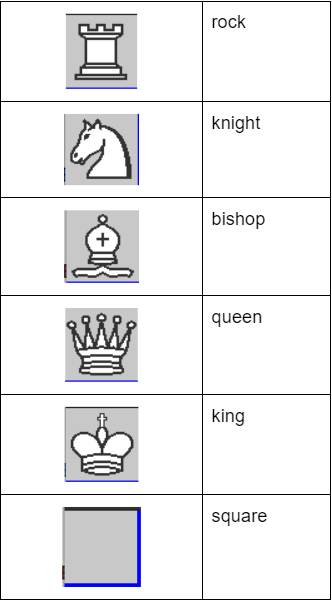
\includegraphics[width=0.5\textwidth, keepaspectratio]{img/figuras.png}
    \caption{Figuras Ajedrez}
  \end{figure}
  \newpage
  
  Estos objetos estarán disponibles importando la biblioteca: chessPictures y estarán internamente representados con arreglos de strings 
  que podrá revisar en el archivo pieces.py

  La clase \textbf{Picture} tiene un sólo atributo: el arreglo de strings img, el cual contendrá la representación en caracteres de la figura 
  que se desea dibujar. 
  
  La clase \textbf{Picture} ya cuenta con una función implementada, no debe modificarla, pero si puede usarla para implementar sus otras funciones:
  \begin{itemize}
    \item \textbf{invColor:} recibe un color como un carácter de texto y devuelve su color negativo, también como texto, deberá revisar el archivo colors.py 
    para conocer los valores negativos de cada carácter.
  \end{itemize}
  La clase textbf{Picture} contará además con varios métodos que usted deberá implementar:
  \begin{enumerate}
    \item \textbf{verticalMirror:} Devuelve el espejo vertical de la imágen.
    \item \textbf{horizontalMirror:} Devuelve el espejo horizontal de la imágen. 
    \item \textbf{negative:} Devuelve un negativo de la imágen.
    \item \textbf{join:} Devuelve una nueva figura poniendo la figura del argumento al lado derecho de la figura actual.
    \item \textbf{up:} Devuelve una nueva figura poniendo la figura recibida como argumento, encima de la figura actual.
    \item \textbf{under:} Devuelve una nueva figura poniendo la figura recibida como argumento, sobre la figura actual.
    \item \textbf{horizontalRepeat:} Devuelve una nueva figura repitiendo la figura actual al costado la cantidad de veces que indique el valor de n.
    \item \textbf{verticalRepeat} Devuelve una nueva figura repitiendo la figura actual debajo, la cantidad de veces que indique el valor de n.
  \end{enumerate}
  Tenga en cuenta que para implementar todos estos métodos, sólo deberá trabajar sobre la representación interna de un Picture, es decir 
  su atributo img.

  Para dibujar una objeto Picture bastará importar el método draw de la biblioteca interpreter y usarlo de la siguiente manera:
  \begin{figure}[H]
    \centering
    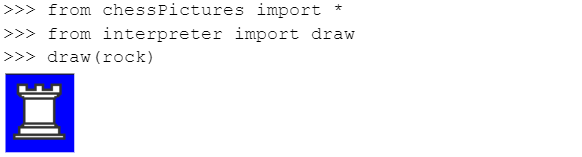
\includegraphics[width=1\textwidth, keepaspectratio]{img/considerar.png}
    \caption{Forma de graficar}
  \end{figure}
  \newpage
  
%%%%%%%%%%%%%
  
  \subsection{Ejercicios}
  Para resolver los siguientes ejercicios \textbf{sólo está permitido usar ciclos, condicionales, definición de listas por comprensión, sublistas, 
  map, join, (+), lambda, zip, append, pop, range.}
  \begin{enumerate}
    \item Implemente los métodos de la clase Picture. Se recomienda que implemente la clase picture por etapas, probando realizar los dibujos que se 
    muestran en la siguiente preguntas.
    \item Usando únicamente los métodos de los objetos de la clase Picture dibuje las siguientes figuras (invoque a draw):
    \begin{figure}[H]
      \centering
      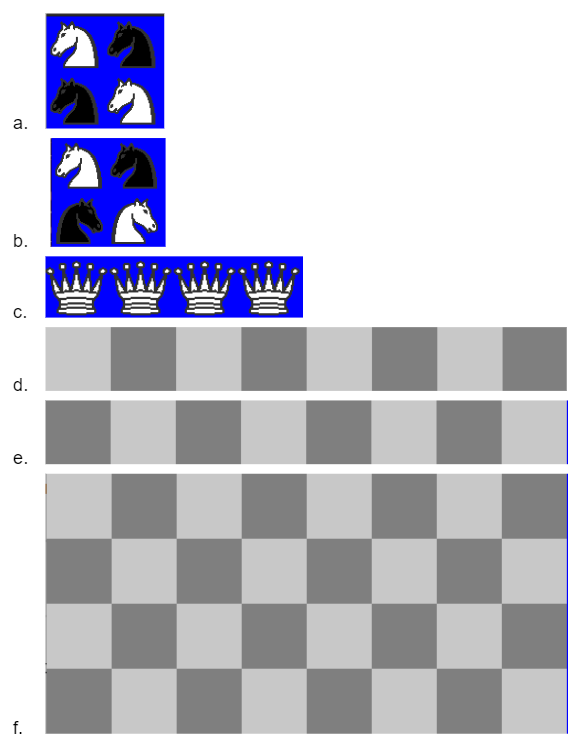
\includegraphics[width=0.4\textwidth, keepaspectratio]{img/ejerciciosP.png}
      \caption{Ejercicios parte 1}
    \end{figure}
    \begin{figure}[H]
      \centering
      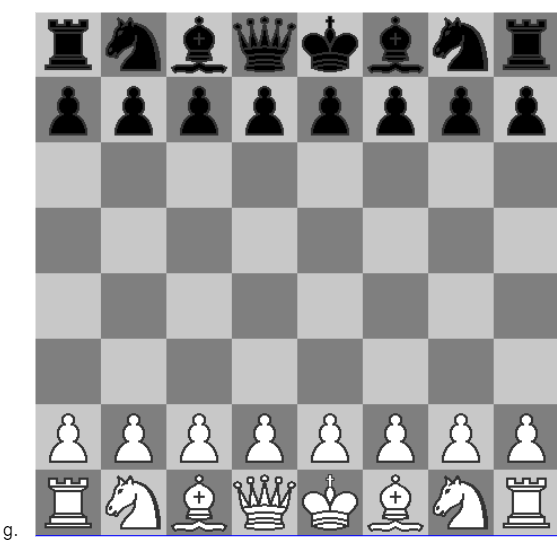
\includegraphics[width=0.4\textwidth, keepaspectratio]{img/ejerciciosP2.png}
      \caption{Ejercicios parte 2}
    \end{figure}
  \end{enumerate}
  \newpage
  
%%%%%%%%%%%%%%%%%%%% 
 
  \section{Entregables}
  \begin{itemize}
    \item Informe en Latex.
    \item URL: Repsotorio de GitHub.
    \item URL: Vídeo Explicativo(Youtube).
  \end{itemize}
  
%%%%%%%%%%%%%%%%%%%%    
		
	\section{Equipos, materiales y temas utilizados}
  \begin{itemize}
    \item Python
    \item Pip
    \item Pygame
    \item Virtual Environment
    \item GitHub
    \item Listas
    \item Ciclos
    \item Consicionales
  \end{itemize}
 
%%%%%%%%%%%%%%%%%%%%

  \section{URL de Repositorio Github}
  \begin{itemize}
    \item Link Repositorio GitHub
    \item \url{https://github.com/Victor-Gonzalo-Maldonado-Vilca/TareaAjedrez_Lab05.git}
  \end{itemize}
    
%%%%%%%%%%%%%%%%%%%%

  \section{Link de Video}
  \begin{itemize}
    \item Link del Vídeo de Youtube
    \item \url{https://www.youtube.com/watch?v=PpSnn4hmAWU}
  \end{itemize}

%%%%%%%%%%%%%

  \begin{figure}[H]
    \centering
    
\includegraphics[width=0.4\textwidth, keepaspectratio]{img/python.png}
    \caption{Python}
  \end{figure}
  \newpage
  
%%%%%%%%%%%%%%%%%%%%

  \section{Metodología}
  
%%%%%%%%%%%%%

  \subsection{Instalación de Python}
  \begin{enumerate}
    \item \textbf{Abrir Microsoft Store:}
    \begin{figure}[H]
      \centering
      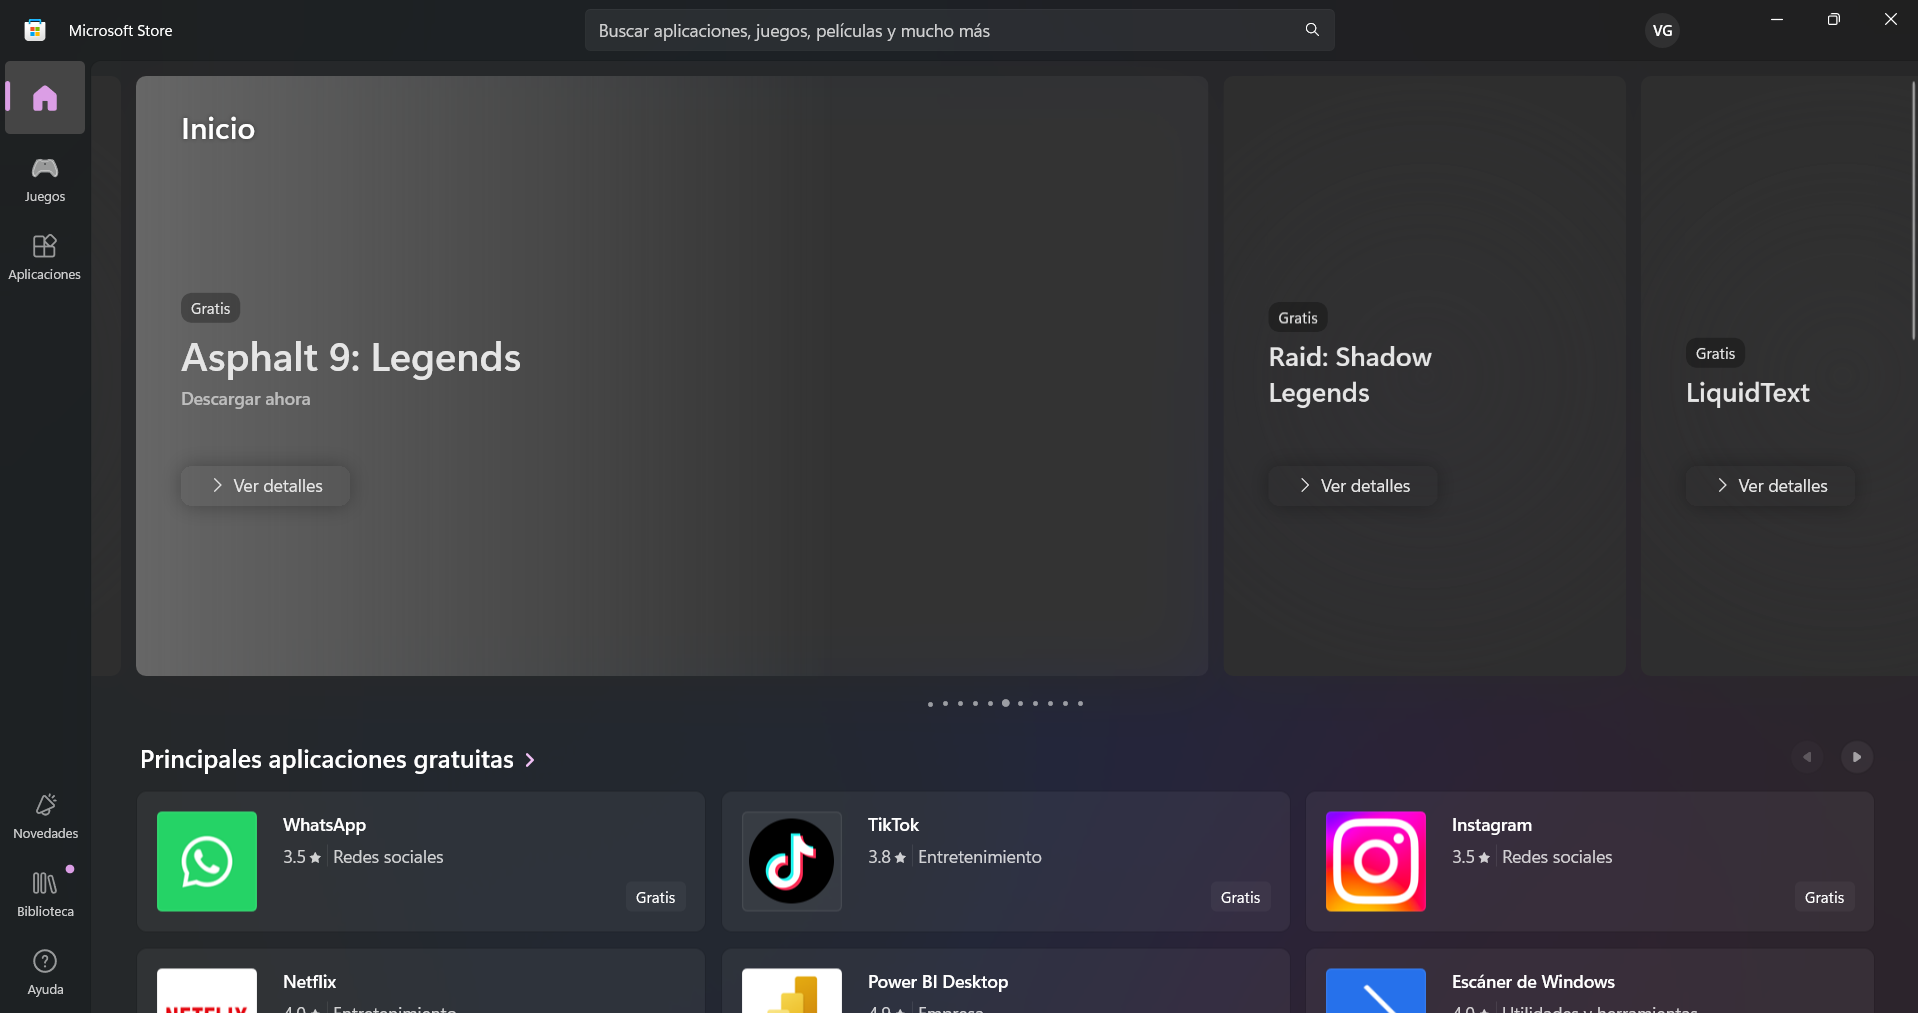
\includegraphics[width=1\textwidth, keepaspectratio]{img/store.png}
      \caption{Microsoft Store}
    \end{figure}
    \item \textbf{Buscar Python:}
    \begin{figure}[H]
      \centering
      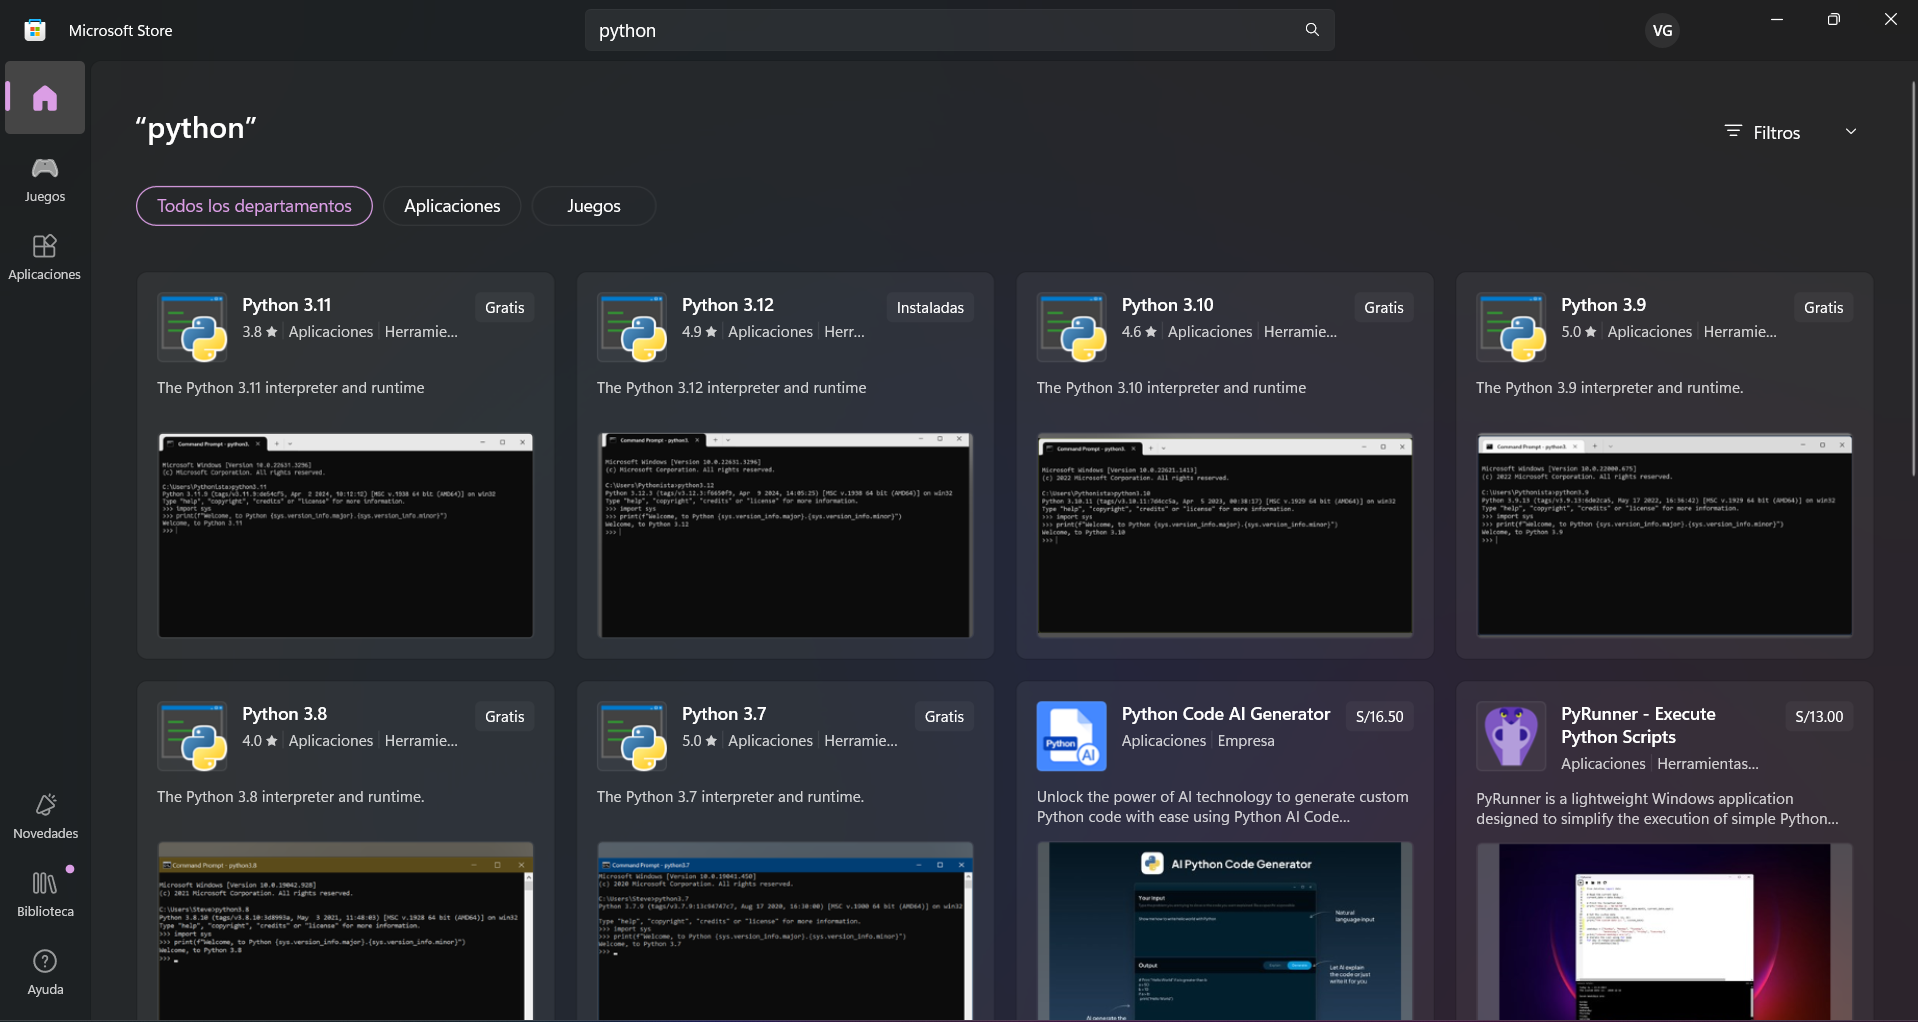
\includegraphics[width=1\textwidth, keepaspectratio]{img/storePython.png}
      \caption{Microsoft Store Python}
    \end{figure}
    \newpage
    \item \textbf{Instalar Python:}
    \begin{figure}[H]
      \centering
      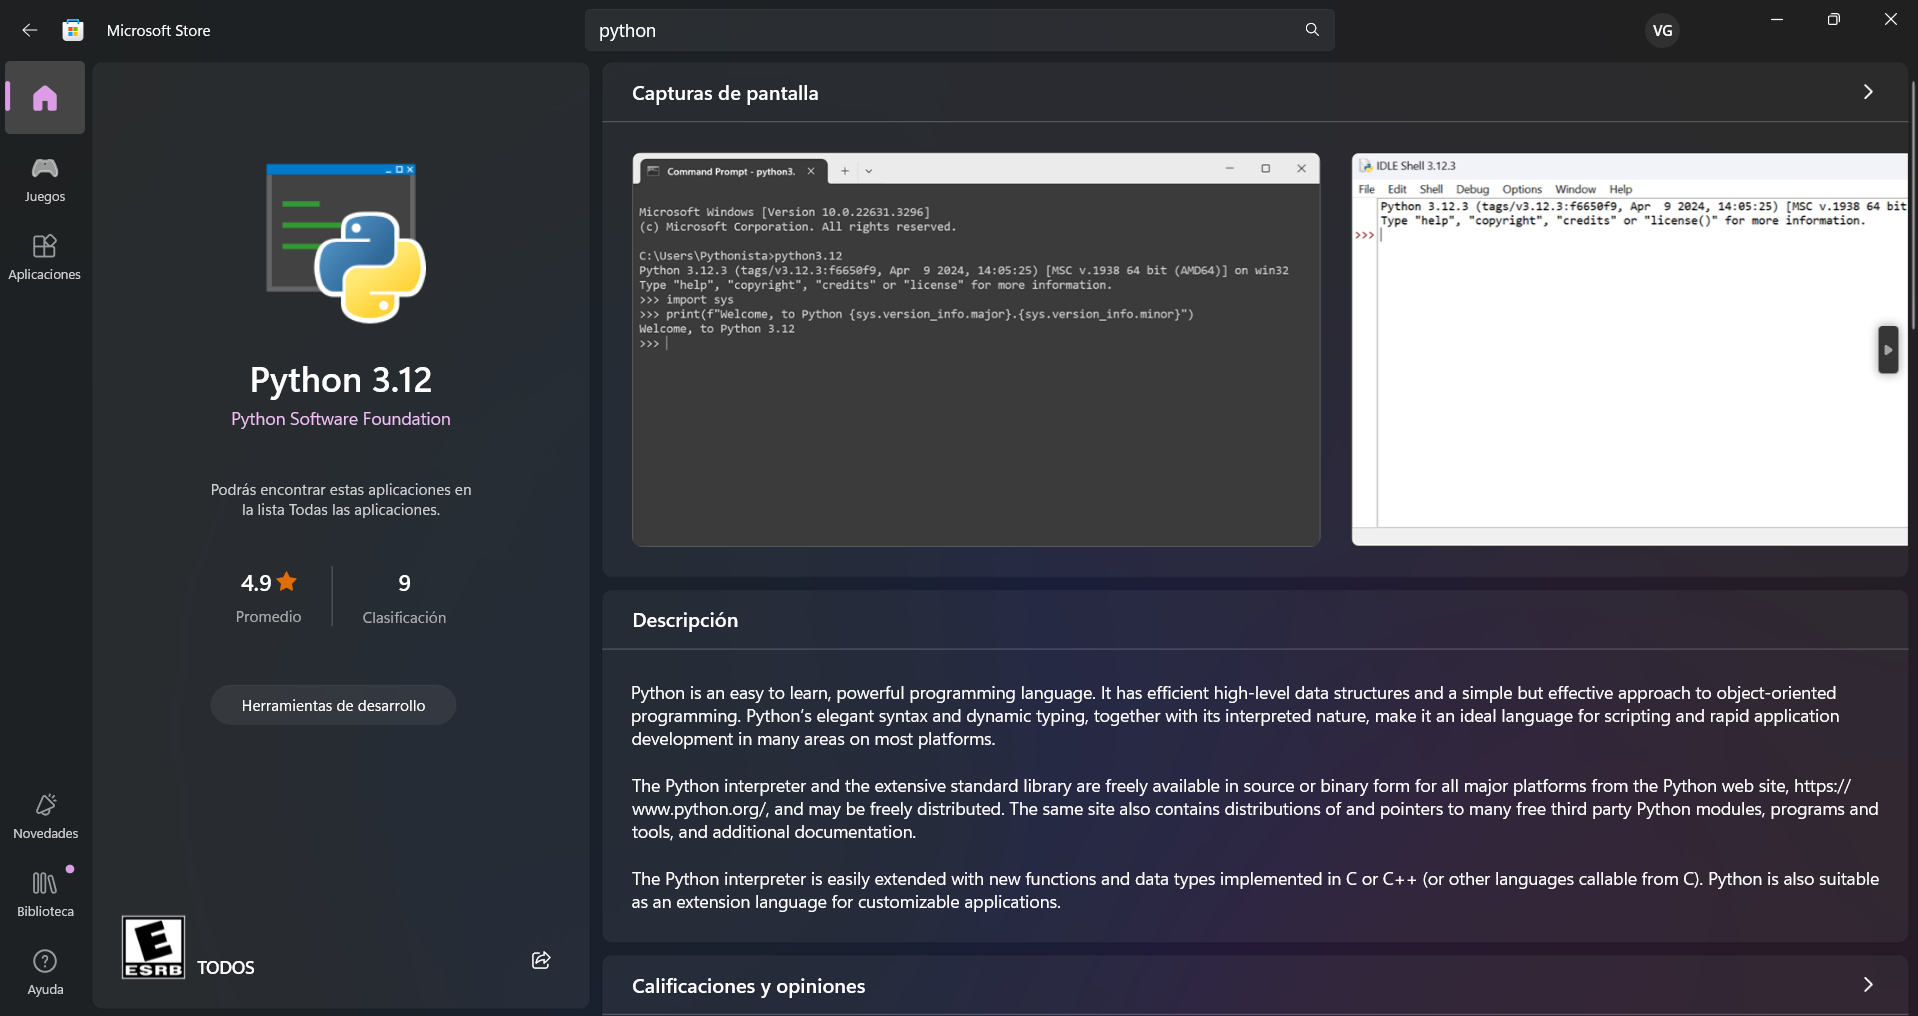
\includegraphics[width=1\textwidth, keepaspectratio]{img/installPython.png}
      \caption{Instalar Python}
    \end{figure}
    \item \textbf{Verificar si se instalo correctamente:} Usamos CMD para verificar.
    \begin{lstlisting}[language={}]
      python --version
    \end{lstlisting}
  \end{enumerate}
  
%%%%%%%%%%%%%

  \subsection{Crear entorno de trabajo}
  
%%%%%%  
  
  \subsubsection{Creación carpetas de Trabajo}
  \begin{itemize}
    \item \textbf{Carpeta lab04\textit{(Se usará para installar pygame y crear entorno virtual)}: }usando comando:
    \begin{lstlisting}[language={}]
      mkdir lab04 && cd lab04
    \end{lstlisting}
    \item \textbf{Carpeta src \textit{(Se usará para los archivos que se requieren en el laboratorio, de igual manera los ejercicios correspondientes)}: }
    estando en el directorio \textbf{lab04} se usa el comando:
    \begin{lstlisting}[language={}]
      mkdir src && cd src
    \end{lstlisting}
  \end{itemize}
  
%%%%%%

  \subsubsection{Uso de Pip para installar virtalenv \textit{(Carpeta Lab04)}}
  \begin{itemize}
    \item \textbf{Verificación de tener pip, comando:}
    \begin{lstlisting}[language={}]
      pip --version
    \end{lstlisting}
    \newpage
    \item \textbf{Uso de comando pip (en mi caso ya lo tenía instalado), comando:}
    \begin{lstlisting}[language={}]
      pip install virtualenv
    \end{lstlisting}
    \item \textbf{Crear entorno virtual usando virtualenv, comando: }
    \begin{lstlisting}[language={}]
      virtualenv -p python3 .
    \end{lstlisting}
  \end{itemize}
  
%%%%%%

  \subsubsection{Inicializar Git \textit{(Carpeta src)}}
  \begin{itemize}
    \item \textbf{Uso del comando:}
    \begin{lstlisting}[language={}]
        git init
    \end{lstlisting}
  \end{itemize}
  
%%%%%%%%%%%%%

  \subsection{Activar entorno Virtual \textit{(Carpeta lab04)}}
  \begin{itemize}
    \item \textbf{En Linux:}
    \begin{lstlisting}[language={}]
      source ../bin/activate
    \end{lstlisting}
    \item \textbf{En Windows:}
    \begin{lstlisting}[language={}]
      ../Scripts/activate
    \end{lstlisting}
  \end{itemize}
  
%%%%%%%%%%%%%  
  
  \subsection{Obtener clases(Picture, chessPicture, etc) de Python}
  \begin{itemize}
    \item Ir al Repositorio entregado por el Docente.
    \begin{figure}[H]
      \centering
      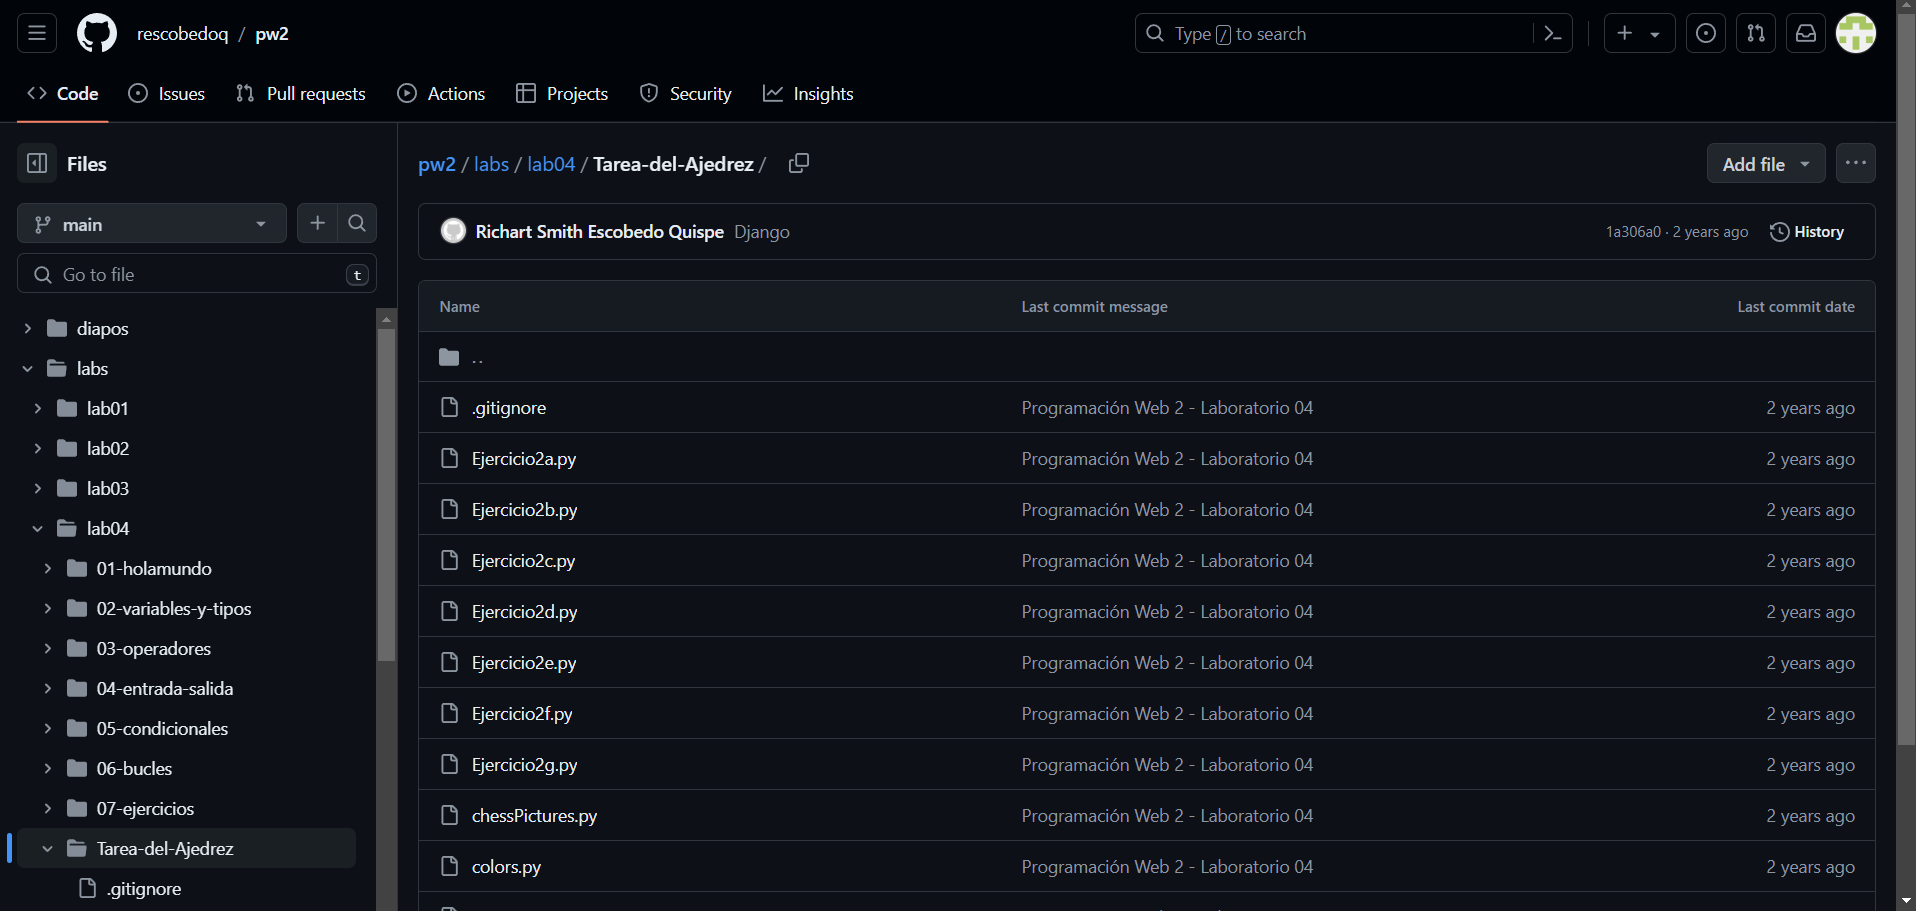
\includegraphics[width=1\textwidth, keepaspectratio]{img/repoDocente.png}
      \caption{Repositorio Docente}
    \end{figure}
    \item Descargar los archivos necesarios en la carpeta src.
  \end{itemize}
  \newpage
%%%%%%%%%%%%%
  
  \subsection{Instalar Pygame}
  \begin{itemize}
    \item Usar comando:
    \begin{lstlisting}[language={}]
      pip install pygame
    \end{lstlisting}
  \end{itemize}
  
%%%%%%%%%%%%%
  
  \subsection{Desactivar entorno Virtual}
  \begin{itemize}
    \item Cuando ya se haya dejado de trabajar en el entorno usamos el comando:
    \begin{lstlisting}[language={}]
      deactivate
    \end{lstlisting}
  \end{itemize}

%%%%%%%%%%%%%%%%%%%%

  \section{Desarrollo del trabajo}

%%%%%%%%%%%%%%%%%%%%

  \subsection{Probando funcionamiento de chessPictures y del interprete}
  \begin{itemize}
    \item \textbf{Prueba 1:}
    \begin{lstlisting}[language=Python, caption=Código de prueba Python]
      from chessPictures import *
      from interpreter import draw
      x = rock
      draw(x)
    \end{lstlisting}
    \begin{figure}[H]
      \centering
      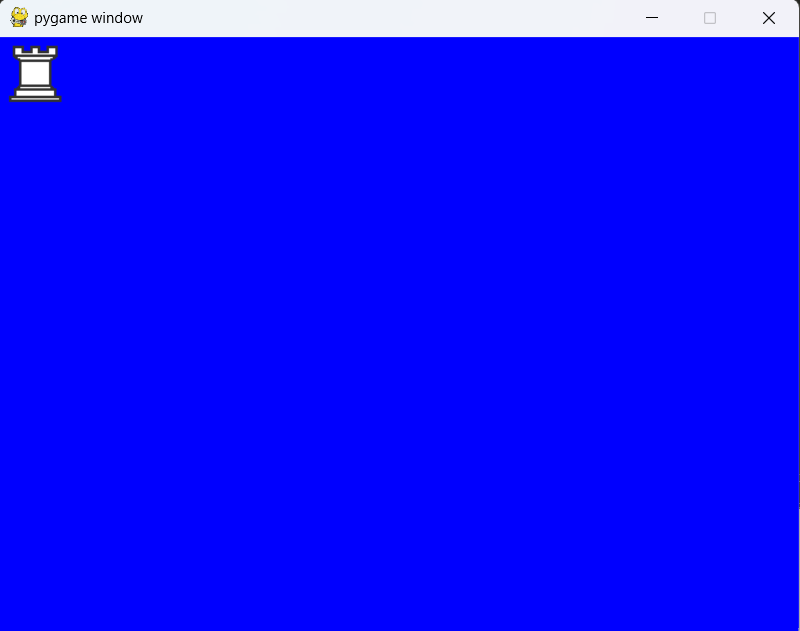
\includegraphics[width=0.7\textwidth, keepaspectratio]{img/prueba1.png}
      \caption{prueba 1}
    \end{figure}
  \end{itemize}
  \newpage
  
%%%%%%%%%%%%

  \subsection{Probando método Vertical Mirror}
  \begin{itemize}
    \item \textbf{Prueba 2 \textit(Vertical Mirror):}
    \begin{lstlisting}[language=Python, caption=Código de prueba Python (ERROR)]
      from chessPictures import *
      from interpreter import draw
      x = verticalMirror(rock)
      draw(x)
    \end{lstlisting}
    \item \textbf{Prueba 3 \textit(Vertical Mirror):}
    \begin{lstlisting}[language=Python, caption=Código de prueba Python (ERROR)]
      from chessPictures import *
      from interpreter import draw
      x = Picture.rock.verticalMirror()
      draw(x)
    \end{lstlisting}
    \item \textbf{Prueba 4 \textit{Vertical Mirror}:}
    \textbf{NORMAL:}
    \begin{lstlisting}[language=Python, caption=Código de prueba Python]
      from chessPictures import *
      from interpreter import draw
      x = knight
      draw(x)
    \end{lstlisting}
    \begin{figure}[H]
      \centering
      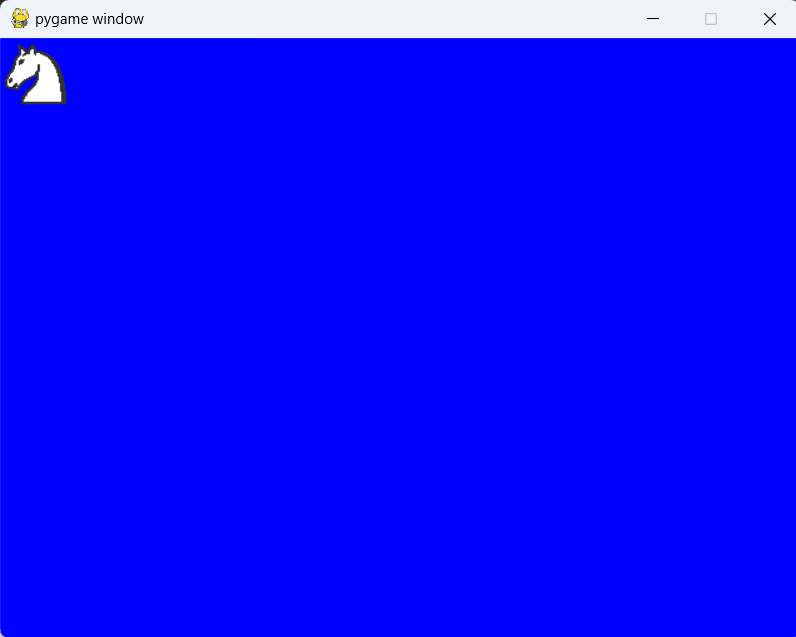
\includegraphics[width=0.7\textwidth, keepaspectratio]{img/normal.png}
      \caption{prueba 4}
    \end{figure}
    \newpage
    \textbf{VERTICAL MIRROR:}
    \begin{lstlisting}[language=Python, caption=Código de prueba Python]
      from chessPictures import *
      from interpreter import draw
      x = rock.verticalMirror()
      draw(x)
    \end{lstlisting}
    \begin{figure}[H]
      \centering
      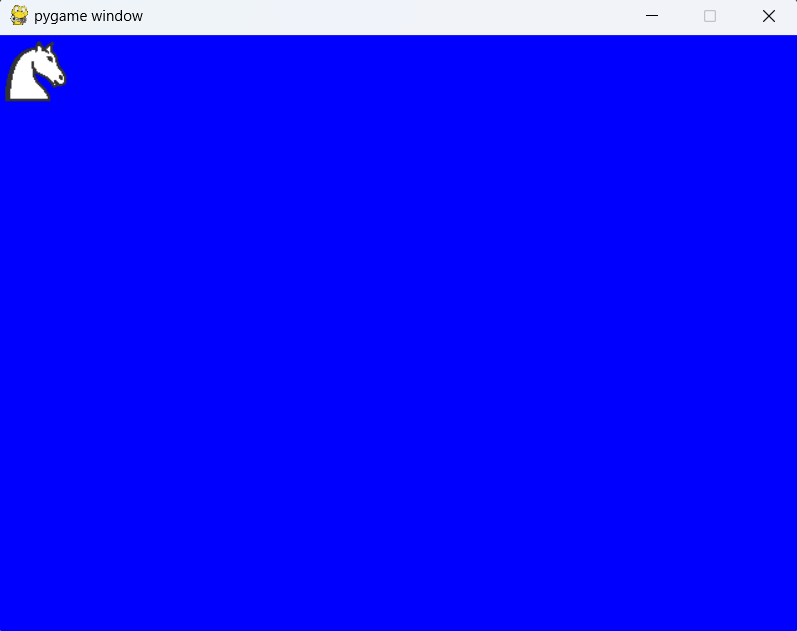
\includegraphics[width=0.7\textwidth, keepaspectratio]{img/vertical.png}
      \caption{prueba 4}
    \end{figure}
  \end{itemize}
  
%%%%%%%%%%%%

  \subsection{Implementación de los Métodos en la clase Picture:}
  
%%%%%%

  \subsubsection{horizontalMirror()}
  \begin{itemize}
    \item \textbf{Descripción: } El método horizontalMirror devuelve la imagen reflejada horizontalmente 
      de una imagen representada por la lista self.img. Itera sobre los elementos de self.img, los agrega en 
      orden inverso a una nueva lista llamada horizontal, y retorna esta lista como una imagen reflejada horizontalmente.
    \item \textbf{Código - sin definición de Listas por Comprensión:}
    \begin{lstlisting}[language=Python, caption=Método horizontalMirror()]
      def horizontalMirror(self):
        """ Devuelve el espejo horizontal de la imagen """
        horizontal = []
        longitud = len(self.img)
        for i in range (longitud):
          horizontal.append(self.img[longitud - i - 1])
        return Picture(horizontal)
    \end{lstlisting}
    \newpage
    \item \textbf{Código - con definición de Listas por Comprensión:}
    \begin{lstlisting}[language=Python, caption=Método horizontalMirror()]
      def horizontalMirror(self):
        """ Devuelve el espejo horizontal de la imagen """
        longitud = len(self.img)
        horizontal = [self.img[longitud - i - 1] for i in range (longitud)]
        return Picture(horizontal)
    \end{lstlisting}
    \item \textbf{Ejecución:}
    \begin{lstlisting}[language=Python, caption=Prueba de horizontalMirror()]
      from chessPictures import *
      from interpreter import draw
      x = rock.horizontalMirror()
      draw(x)
    \end{lstlisting}
    \begin{figure}[H]
      \centering
      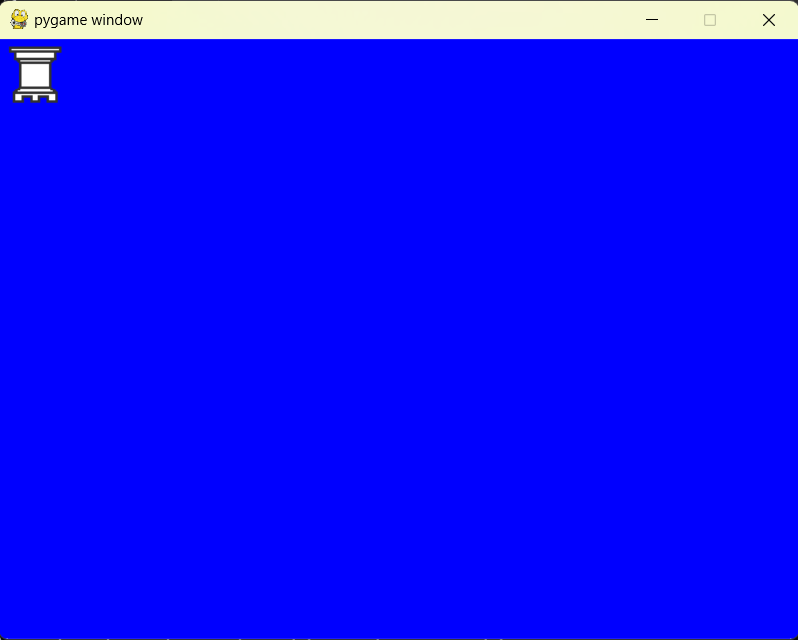
\includegraphics[width=0.8\textwidth, keepaspectratio]{img/horizontal.png}
      \caption{Método horizontalMirror()}
    \end{figure}
  \end{itemize}
  
%%%%%%

  \subsubsection{negative()}
  \begin{itemize}
    \item \textbf{Descripción: }Este método negative retorna el negativo de una imagen representada 
      por la lista self.img. Recorre cada fila de la imagen, luego cada píxel en esa fila, invierte su color utilizando la 
      función invColor, y agrega el píxel invertido a una nueva fila en la lista negativo. 
      \newpage
      Finalmente, devuelve una nueva imagen representada por la lista negativo, que es el negativo de la imagen original. 
      En resumen, este método genera el negativo de una imagen al invertir los colores de todos los píxeles en cada fila de la imagen.
    \item \textbf{Código - sin definición de Listas por Comprensión:}
    \begin{lstlisting}[language=Python, caption=Método negative()]
      def negative(self):
        """ Devuelve un negativo de la imagen """
        negativo = []
        for value in self.img:
          valueNegative = ""
          for i in range(len(value)):
            valueNegative += self._invColor(value[i])
          negativo.append(valueNegative)
        return Picture(negativo)
    \end{lstlisting}
    \item \textbf{Código - con definición de Listas por Comprensión:}
    \begin{lstlisting}[language=Python, caption=Método negative()]
      def negative(self):
        """ Devuelve un negativo de la imagen """
        negativo = [''.join(self._invColor(pixel) for pixel in value) for value in self.img]
        return Picture(negativo)
    \end{lstlisting}
    \item \textbf{Ejecución:}
    \begin{lstlisting}[language=Python, caption=Prueba de negative()]
      from chessPictures import *
      from interpreter import draw
      x = king.negative()
      draw(x)
    \end{lstlisting}
    \begin{figure}[H]
      \centering
      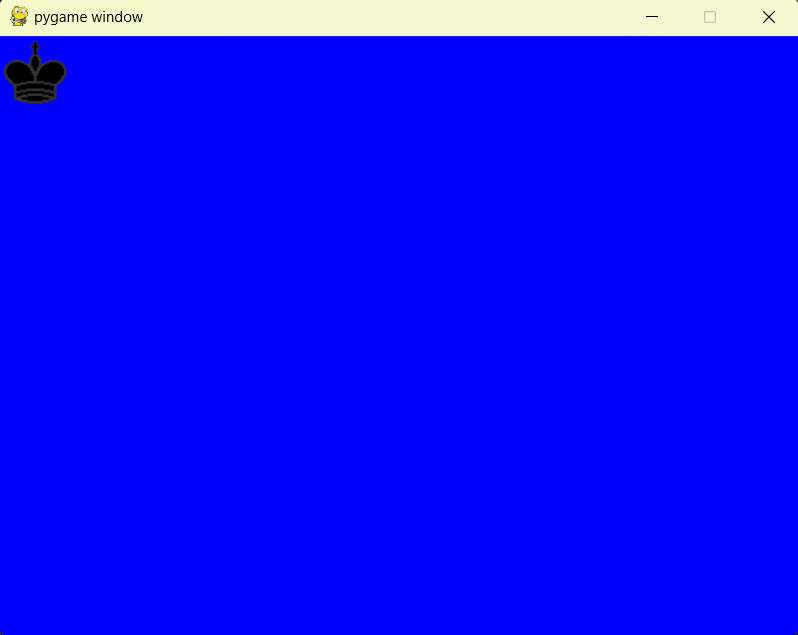
\includegraphics[width=0.8\textwidth, keepaspectratio]{img/negative.png}
      \caption{Método negative()}
    \end{figure}
  \end{itemize}
  
%%%%%%

  \subsubsection{join()}
  \begin{itemize}
    \item \textbf{Descripción: }El método join devuelve una nueva figura que combina la figura actual 
      con otra figura proporcionada como argumento, colocando la figura del argumento al lado derecho de la figura actual. 
      Utiliza la función zip para combinar las filas de ambas figuras y luego une los elementos correspondientes de cada fila 
      mediante la concatenación. Finalmente, crea una nueva imagen con las filas combinadas y la devuelve.
    \item \textbf{Código - sin definición de Listas por Comprensión:}
    \begin{lstlisting}[language=Python, caption=Método join()]
      def join(self, p):
        """ Devuelve una nueva figura poniendo la figura del argumento 
            al lado derecho de la figura actual """
        alado = []
        i = 0
        for value in self.img:
          alado.append(value)
        for value in p.img:
          alado[i] += value
          i += 1
        return Picture(alado)
    \end{lstlisting}
    \newpage
    \item \textbf{Código - con definición de Listas por Comprensión:}
    \begin{lstlisting}[language=Python, caption=Método join()]
      def join(self, p):
        """ Devuelve una nueva figura poniendo la figura del argumento 
            al lado derecho de la figura actual """
        alado = [value1 + value2 for value1,value2 in zip(self.img,p.img)]
        return Picture(alado)
    \end{lstlisting}
    \item \textbf{Ejecución:}
    \begin{lstlisting}[language=Python, caption=Prueba de join()]
      from chessPictures import *
      from interpreter import draw
      x = queen.join(square)
      draw(x)
    \end{lstlisting}
    \begin{figure}[H]
      \centering
      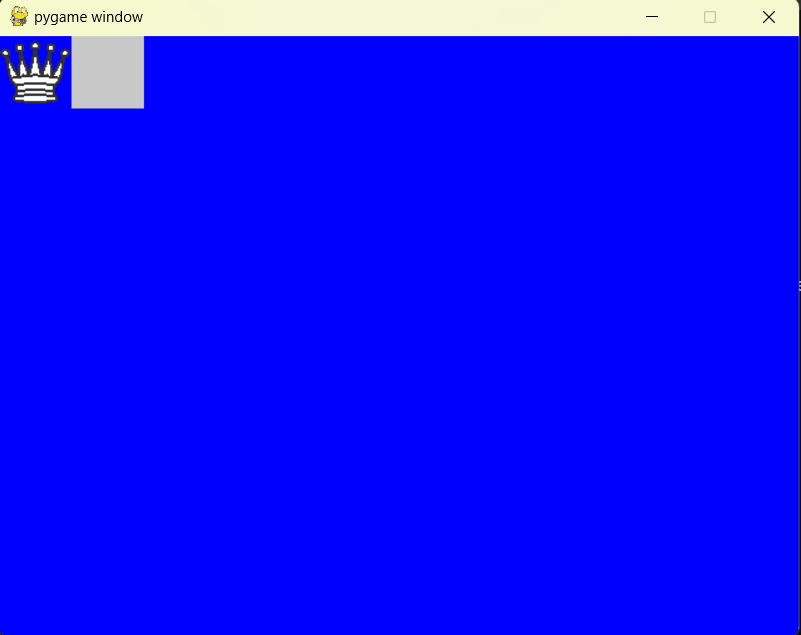
\includegraphics[width=0.8\textwidth, keepaspectratio]{img/join.png}
      \caption{Método join()}
    \end{figure}
  \end{itemize}
  
%%%%%%

  \subsubsection{up()}
  \begin{itemize}
    \item \textbf{Descripción: }La función up de la clase Picture toma otra instancia de Picture 
      como parámetro, representada por p. Internamente, combina las imágenes de la instancia actual y la instancia p, 
      colocando la imagen de p encima de la imagen de la instancia actual. Luego, devuelve un nuevo objeto Picture con 
      esta combinación de imágenes.
    \newpage
    \item \textbf{Código: }
    \begin{lstlisting}[language=Python, caption=Método up()]
      def up(self, p):
        encima = p.img + self.img
        return Picture(encima)
    \end{lstlisting}
    \item \textbf{Ejecución:}
    \begin{lstlisting}[language=Python, caption=Prueba up()]
      from chessPictures import *
      from interpreter import draw
      x = queen.up(rock)
      draw(x)
    \end{lstlisting}
    \begin{figure}[H]
      \centering
      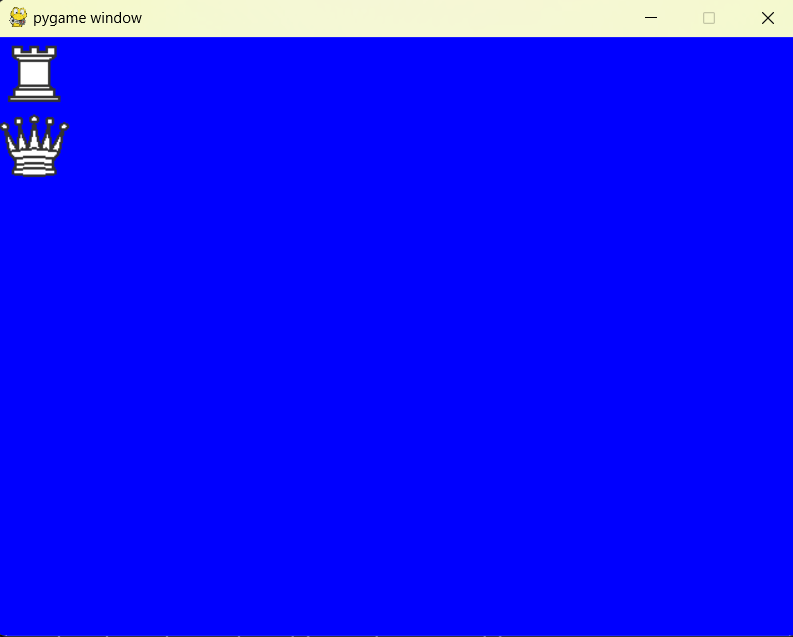
\includegraphics[width=0.8\textwidth, keepaspectratio]{img/up.png}
      \caption{Método up()}
    \end{figure}
  \end{itemize}
  
%%%%%%

  \subsubsection{under()}
  \begin{itemize}
    \item \textbf{Descripción: }El método under de la clase Picture crea una nueva imagen colocando la 
      imagen de otro objeto Picture sobre la imagen de la instancia actual. Si las imágenes no tienen la misma longitud, 
      simplemente devuelve la imagen del objeto Picture pasado como argumento. En caso contrario, combina las imágenes superponiendo 
      los píxeles de ambas imágenes y retorna un nuevo objeto Picture con esta composición.
    \newpage
    \item \textbf{Código - sin definición de Listas por Comprensión:}
    \begin{lstlisting}[language=Python, caption=Método under()]
      def under(self, p):
        """ Devuelve una nueva figura poniendo la figura p sobre la
            figura actual """
        sobre = []
        if(len(p.img) != len(self.img)):
          return Picture(p.img)
        for value1,value2 in zip(self.img,p.img):
          cadena = ""
          for i in range(len(value1)):
            if(value2[i] == ' '):
              cadena += value1[i]
            else:
              cadena += value2[i]
          sobre.append(cadena)
        return Picture(sobre)
    \end{lstlisting}
    \item \textbf{Código - con definición de Listas por Comprensión:}
    \begin{lstlisting}[language=Python, caption=Método under()]
      def under(self, p):
        """ Devuelve una nueva figura poniendo la figura p sobre la
            figura actual """
        sobre = [''.join(value1[i] if value2[i] == ' ' else value2[i] for i in range(len(value1))) for value1,value2 in zip(self.img,p.img)]
        return Picture(sobre) if len(self.img) == len(p.img) else Picture(p.img)
    \end{lstlisting}
    \item \textbf{Ejecución:}
    \begin{lstlisting}[language=Python, caption=Prueba under()]
      from chessPictures import *
      from interpreter import draw
      x = square.under(rock)
      draw(x)
    \end{lstlisting}
    \begin{figure}[H]
      \centering
      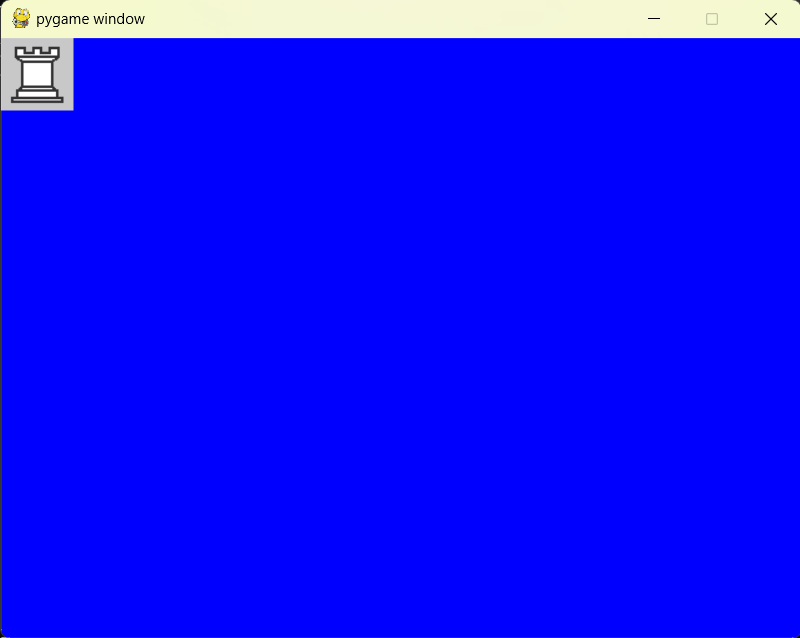
\includegraphics[width=0.8\textwidth, keepaspectratio]{img/under.png}
      \caption{Método under()}
    \end{figure}
  \end{itemize}
  
%%%%%%

  \subsubsection{horizontalRepeat()}
  \begin{itemize}
    \item \textbf{Descripción: }horizontalRepeat es un método de la clase Picture que devuelve una nueva figura 
      que repite horizontalmente la figura actual un número específico de veces. Para lograr esto, el método toma el número 
      de repeticiones como argumento y construye una nueva figura donde cada fila de la figura original se concatena consigo misma 
      la cantidad de veces especificada. Esto permite crear una nueva figura que tenga la misma forma que la figura original, pero 
      que se extiende horizontalmente según el número de repeticiones especificado.
    \item \textbf{Código - sin definición de Listas por Comprensión:}
    \begin{lstlisting}[language=Python, caption=Método horizontalRepeat()]
      def horizontalRepeat(self, n):
        """ Devuelve una nueva figura repitiendo la figura actual al costado
            la cantidad de veces que indique el valor de n """
        repeath = []
        for value in self.img:
          cadena = ""
          for i in range(n):
            cadena += value
          repeath.append(cadena)
        return Picture(repeath)
    \end{lstlisting}
    \newpage
    \item \textbf{Código - con definición de Listas por Comprensión:}
    \begin{lstlisting}[language=Python, caption=Método horizontalRepeat()]
      def horizontalRepeat(self, n):
        """ Devuelve una nueva figura repitiendo la figura actual al costado
            la cantidad de veces que indique el valor de n """
        repeath = [''.join(value for i in range(n)) for value in self.img]
        return Picture(repeath)
    \end{lstlisting}
    \item \textbf{Ejecución:}
    \begin{lstlisting}[language=Python, caption=Prueba horizontalRepeat()]
      from chessPictures import *
      from interpreter import draw
      x = knight.horizontalRepeat(7)
      draw(x)
    \end{lstlisting}
    \begin{figure}[H]
      \centering
      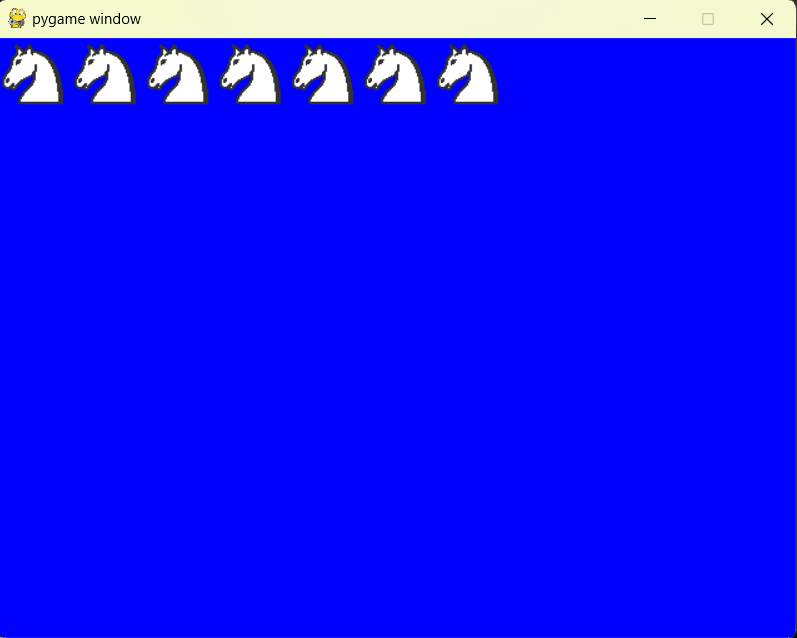
\includegraphics[width=0.8\textwidth, keepaspectratio]{img/repeath.png}
      \caption{Método horizontalRepeat()}
    \end{figure}
  \end{itemize}
  
%%%%%%

  \subsubsection{verticalRepeat()}
  \begin{itemize}
    \item \textbf{Descripción: }verticalRepeat genera una nueva figura replicando verticalmente la figura actual según un número específico de repeticiones. 
      Esto significa que la imagen se apila una encima de la otra, creando una imagen más alta.
    \newpage
    \item \textbf{Código - sin definición de Listas por Comprensión:}
    \begin{lstlisting}[language=Python, caption=Método verticalRepeat()]
      def verticalRepeat(self, n):
        repeatv = []
        for i in range(n):
          for value in self.img:
            repeatv.append(value)
        return Picture(repeatv)
    \end{lstlisting}
    \item \textbf{Código - con definición de Listas por Comprensión:}
    \begin{lstlisting}[language=Python, caption=Método verticalRepeat()]
      def verticalRepeat(self, n):
        repeatv = [value for i in range(n) for value in self.img]
        return Picture(repeatv)
    \end{lstlisting}
    \item \textbf{Ejecución:}
    \begin{lstlisting}[language=Python, caption=Prueba verticalRepeat()]
      from chessPictures import *
      from interpreter import draw
      x = king.verticalRepeat(5)
      draw(x)
    \end{lstlisting}
    \begin{figure}[H]
      \centering
      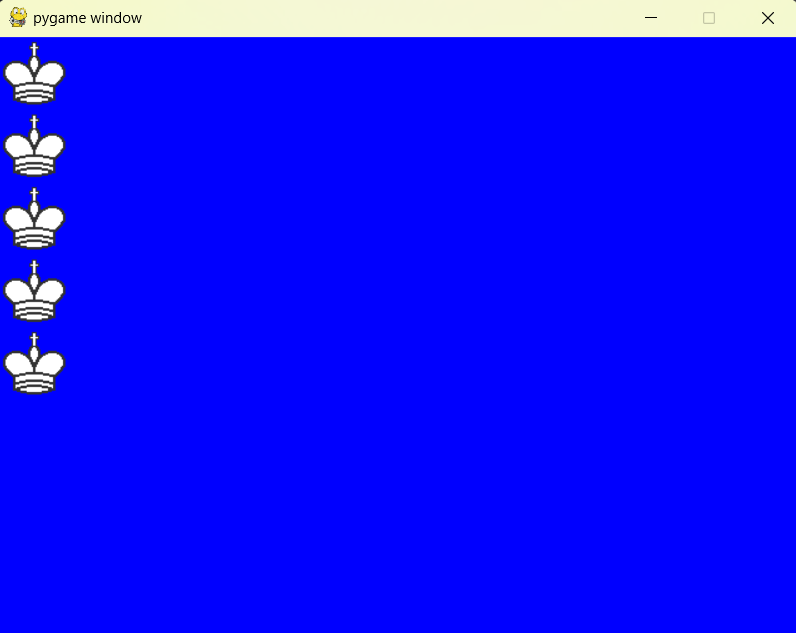
\includegraphics[width=0.8\textwidth, keepaspectratio]{img/repeatv.png}
      \caption{Método verticalRepeat()}
    \end{figure}
  \end{itemize}
  \newpage
  
%%%%%%

  \subsubsection{rotate()}
  \begin{itemize}
    \item \textbf{Descripción: }
      rotate es un método que devuelve una nueva figura rotada en 90 grados. Esto significa que los elementos de la figura se reorganizan 
      de manera que cada fila se convierte en una columna en la nueva figura, y las filas originales se reorganizan en orden inverso.
    \item \textbf{Código - sin definición de Listas por Comprensión:}
    \begin{lstlisting}[language=Python, caption=Método rotate()]
      def rotate(self):
        """Devuelve una figura rotada en 90 grados, puede ser en sentido horario
        o antihorario"""
        rotar = []
        for i in range (len(self.img[0])):
          cadena = ""
          for c in range(len(self.img) -1, -1, -1):
            value = self.img[c]
            cadena += value[i]
          rotar.append(cadena)
        return  Picture(rotar)
    \end{lstlisting}
    \item \textbf{Código - con definición de Listas por Comprensión:}
    \begin{lstlisting}[language=Python, caption=Método rotate()]
      def rotate(self):
        """Devuelve una figura rotada en 90 grados, puede ser en sentido horario
        o antihorario"""
        rotar = [''.join(self.img[c][i] for c in range(len(self.img) - 1, -1, -1)) for i in range(len(self.img[0]))]
        return  Picture(rotar)
    \end{lstlisting}
    \item \textbf{Ejecución:}
    \begin{lstlisting}[language=Python, caption=Prueba rotate()]
      from chessPictures import *
      from interpreter import draw
      x = queen.rotate()
      draw(x)
    \end{lstlisting}
    \newpage
    \begin{figure}[H]
      \centering
      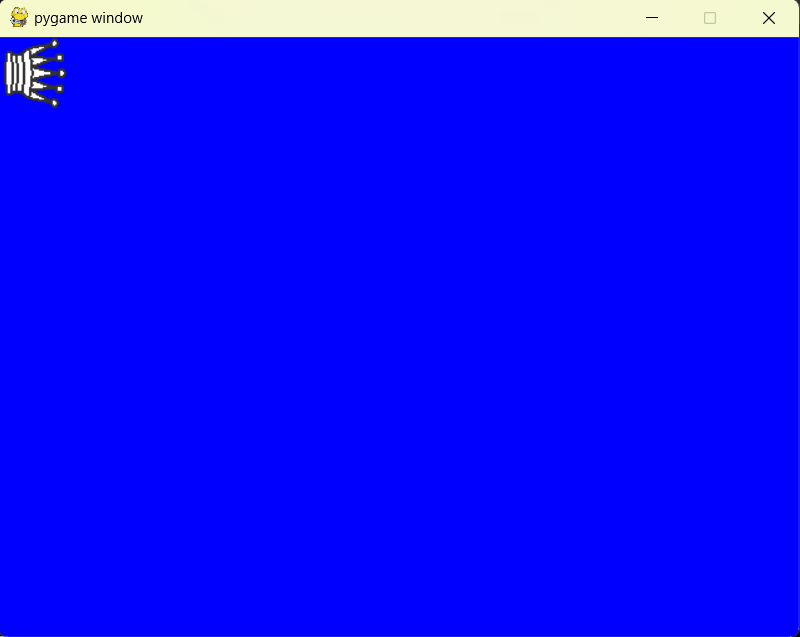
\includegraphics[width=0.8\textwidth, keepaspectratio]{img/rotate.png}
      \caption{Método rotate()}
    \end{figure}
  \end{itemize}

%%%%%%

  \subsubsection{EXTRA: verticalMirror}
  \textit{El Método ya fue implementado por el docente, en está seccion se dará a conocer otra manera de la implementación del Método}
  \begin{itemize}
    \item \textbf{Código - con definición de Listas por Comprensión:}
    \begin{lstlisting}[language=Python, caption=Método verticalMirror()]
      def verticalMirror(self):
        """ Devuelve el espejo vertical de la imagen """
        vertical = [value[::-1] for value in self.img]
        return Picture(vertical)
    \end{lstlisting}
    \item \textbf{Ejecución:}
    \begin{lstlisting}[language=Python, caption=Prueba verticalMirror()]
      from chessPictures import *
      from interpreter import draw
      x = knight.join(rock).verticalMirror()
      draw(x)
    \end{lstlisting}
    \begin{figure}[H]
      \centering
      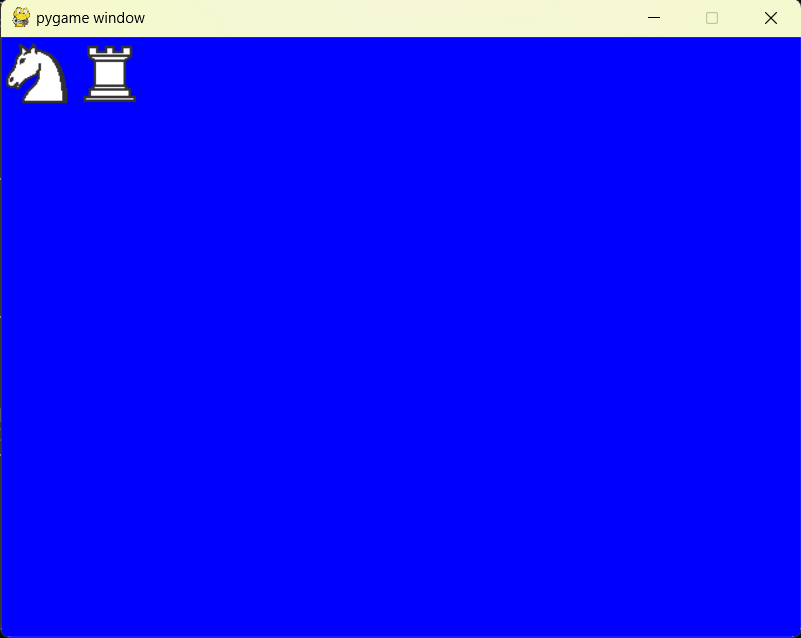
\includegraphics[width=0.7\textwidth, keepaspectratio]{img/normalv.png}
      \caption{Gráfica Normal}
    \end{figure}
    \begin{figure}[H]
      \centering
      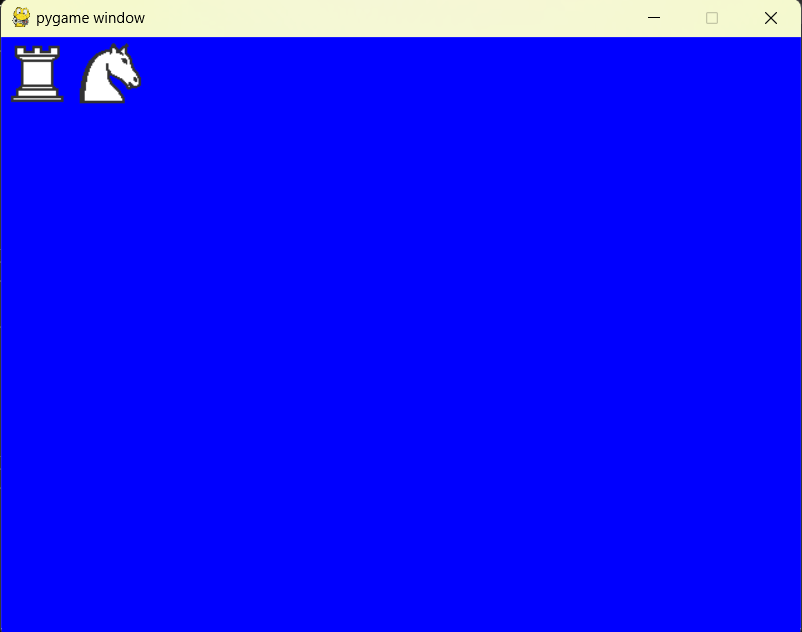
\includegraphics[width=0.7\textwidth, keepaspectratio]{img/vMirror.png}
      \caption{Método verticalMirror()}
    \end{figure}
  \end{itemize}

%%%%%%%%%%%%

  \newpage
  \subsection{EJERCICIOS}
  \textit{Lograr Gráficar las imágenes que se muestran en el documento del Docente}

%%%%%%%

  \subsubsection{Ejercicio 1 (A)}
  \begin{itemize}
    \item \textbf{Código:}
    \begin{lstlisting}[language=Python, caption=Ejercicio2a]
      from interpreter import draw
      from chessPictures import *
      fila = knight.join(knight.negative())
      draw(fila.negative().up(fila))
    \end{lstlisting}
    \item \textbf{Ejecución:}
    \begin{figure}[H]
      \centering
      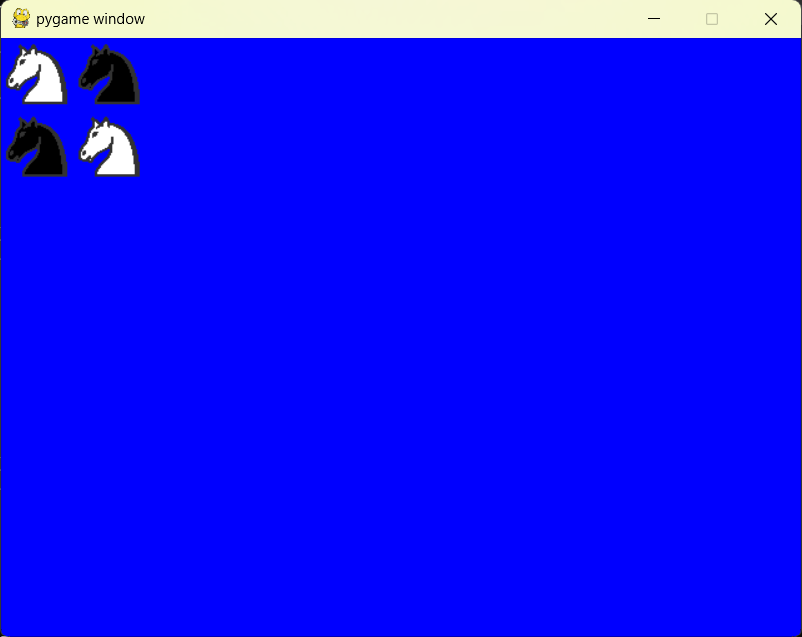
\includegraphics[width=1\textwidth, keepaspectratio]{img/ejercicio2a.png}
      \caption{Ejercicio 1}
    \end{figure}
  \end{itemize}
  \newpage

%%%%%%%

  \subsubsection{Ejercicio 2 (B)}
  \begin{itemize}
    \item \textbf{Código:}
    \begin{lstlisting}[language=Python, caption=Ejercicio2b]
      from interpreter import draw
      from chessPictures import *
      fila = knight.join(knight.negative())
      draw(fila.verticalMirror().up(fila))
    \end{lstlisting}
    \item \textbf{Ejecución:}  
    \begin{figure}[H]
      \centering
      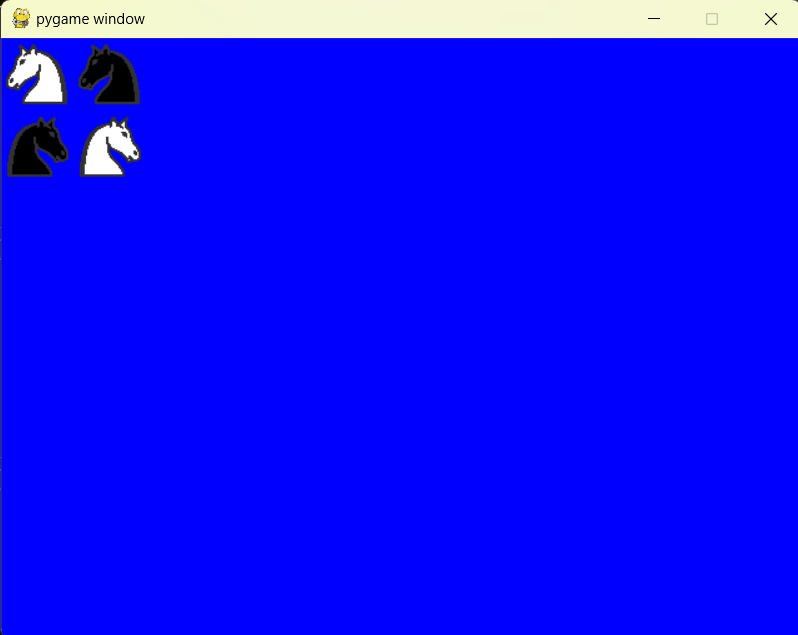
\includegraphics[width=1\textwidth, keepaspectratio]{img/ejercicio2b.png}
      \caption{Ejercicio 2}
    \end{figure}
  \end{itemize}
  \newpage

%%%%%%%

  \subsubsection{Ejercicio 3 (C)}
  \begin{itemize}
    \item \textbf{Código:}
    \begin{lstlisting}[language=Python, caption=Ejercicio2c]
      from interpreter import draw
      from chessPictures import *
      fila = queen.horizontalRepeat(4)
      draw(fila)
    \end{lstlisting}
    \item \textbf{Ejecución:}  
    \begin{figure}[H]
      \centering
      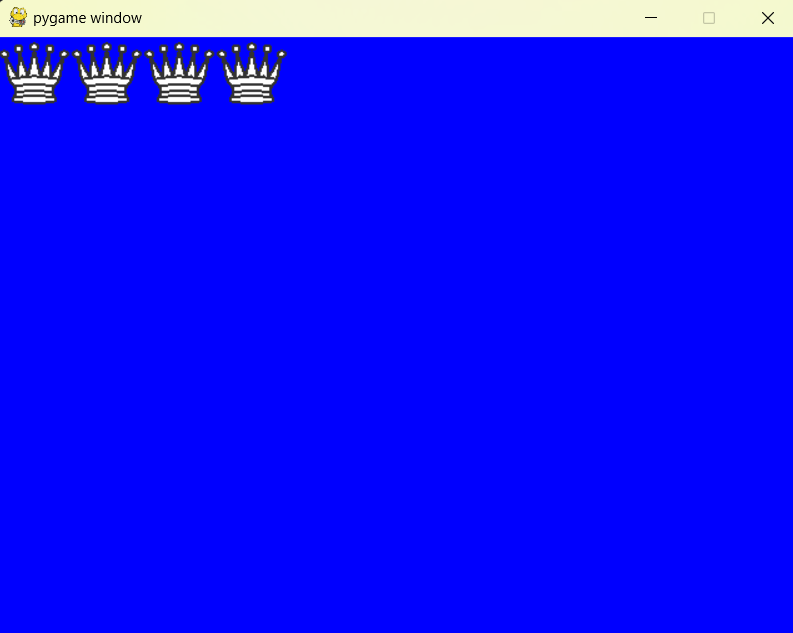
\includegraphics[width=1\textwidth, keepaspectratio]{img/ejercicio2c.png}
      \caption{Ejercicio 3}
    \end{figure}
  \end{itemize}
  \newpage

%%%%%%%

  \subsubsection{Ejercicio 4 (D)}
  \begin{itemize}
    \item \textbf{Código:}
    \begin{lstlisting}[language=Python, caption=Ejercicio2d]
      from interpreter import draw
      from chessPictures import *
      fila = square.join(square.negative()).horizontalRepeat(4)
      draw(fila)
    \end{lstlisting}
    \item \textbf{Ejecución:}  
    \begin{figure}[H]
      \centering
      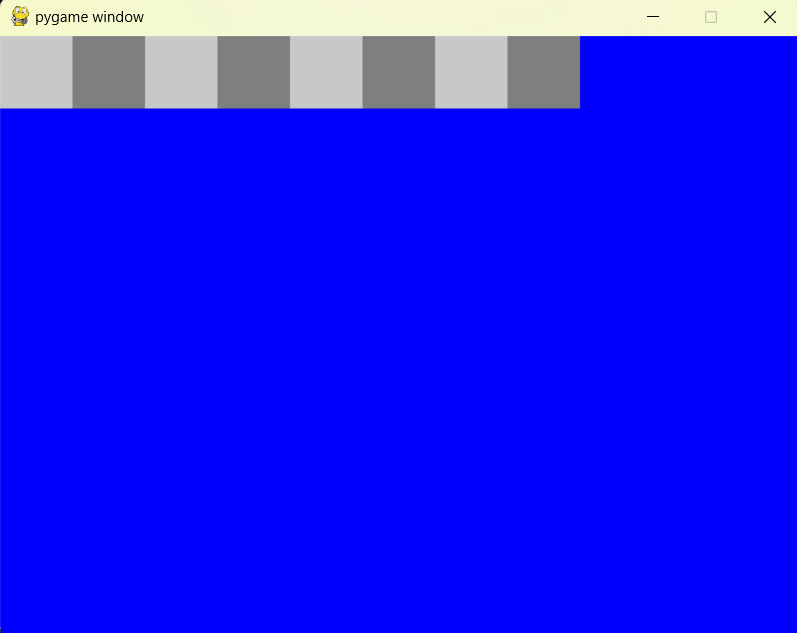
\includegraphics[width=1\textwidth, keepaspectratio]{img/ejercicio2d.png}
      \caption{Ejercicio 4}
    \end{figure}
  \end{itemize}
  \newpage

%%%%%%%

  \subsubsection{Ejercicio 5 (E)}
  \begin{itemize}
    \item \textbf{Código:}
    \begin{lstlisting}[language=Python, caption=Ejercicio2e]
      from interpreter import draw
      from chessPictures import *
      fila = square.join(square.negative()).negative().horizontalRepeat(4)
      draw(fila)
    \end{lstlisting}
    \item \textbf{Ejecución:}  
    \begin{figure}[H]
      \centering
      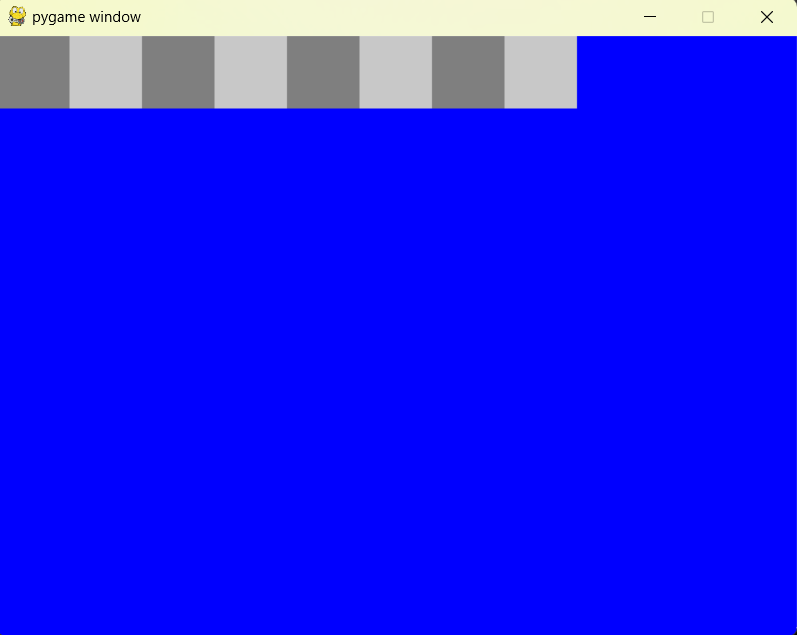
\includegraphics[width=1\textwidth, keepaspectratio]{img/ejercicio2e.png}
      \caption{Ejercicio 5}
    \end{figure}
  \end{itemize}
  \newpage

%%%%%%%

  \subsubsection{Ejercicio 6 (F)}
  \begin{itemize}
    \item \textbf{Código:}
    \begin{lstlisting}[language=Python, caption=Ejercicio2f]
      from interpreter import draw
      from chessPictures import *
      fila = square.join(square.negative()).horizontalRepeat(4)
      draw(fila.negative().up(fila).verticalRepeat(2))
    \end{lstlisting}
    \item \textbf{Ejecución:}  
    \begin{figure}[H]
      \centering
      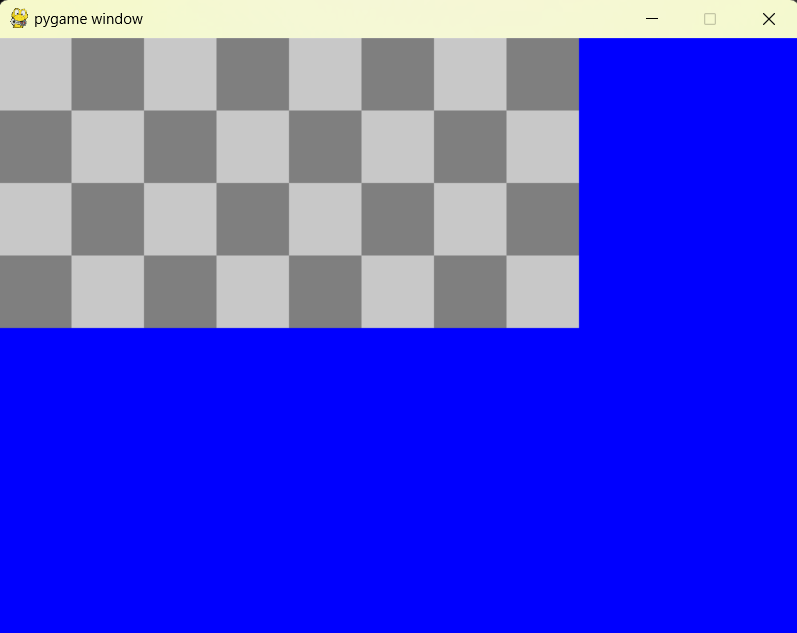
\includegraphics[width=1\textwidth, keepaspectratio]{img/ejercicio2f.png}
      \caption{Ejercicio 6}
    \end{figure}
  \end{itemize}
  \newpage

%%%%%%%

  \subsubsection{Ejercicio 7 (G)}
  \begin{itemize}
    \item \textbf{Código:}
    \begin{lstlisting}[language=Python, caption=Ejercicio2g]
      from interpreter import draw
      from chessPictures import *
      fila = square.join(square.negative()).horizontalRepeat(4)
      fichas = rock.join(knight).join(bishop).join(queen).join(king).join(bishop).join(knight).join(rock)
      peones = pawn.horizontalRepeat(8)
      fichasBlancas = fila.negative().under(fichas).up(fila.under(peones)) 
      fichasNegras = fila.negative().under(peones.negative()).up(fila.under(fichas.negative()))
      tablero = fichasBlancas.up(fila.negative().up(fila).verticalRepeat(2)).up(fichasNegras)
      draw(tablero)
    \end{lstlisting}
    \item \textbf{Ejecución:}  
    \begin{figure}[H]
      \centering
      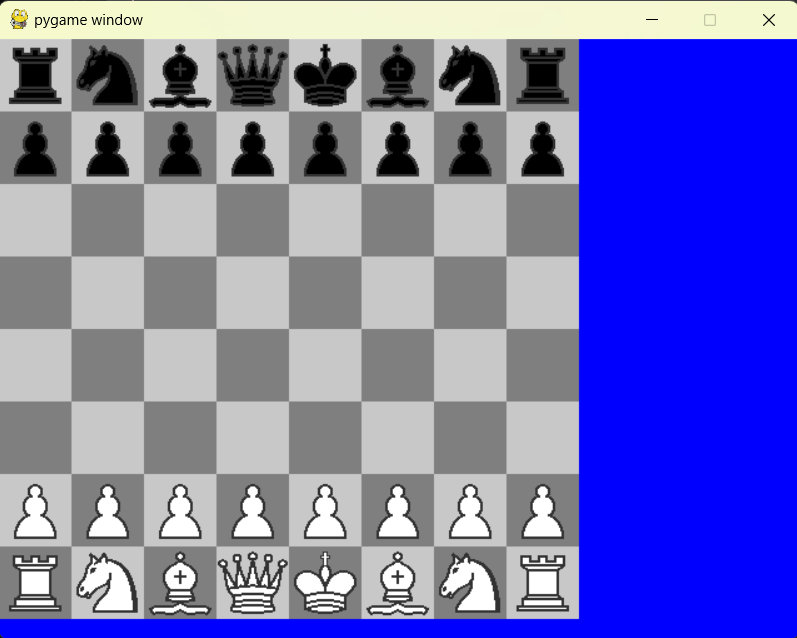
\includegraphics[width=1\textwidth, keepaspectratio]{img/ejercicio2g.png}
      \caption{Ejercicio 7}
    \end{figure}
  \end{itemize}
  \newpage

%%%%%%%%%%%%
	
  \subsection{Uso de GitHub}
  
%%%%%%%

	\subsubsection{Usuario de GitHub}
  \begin{figure}[H]
    \centering
    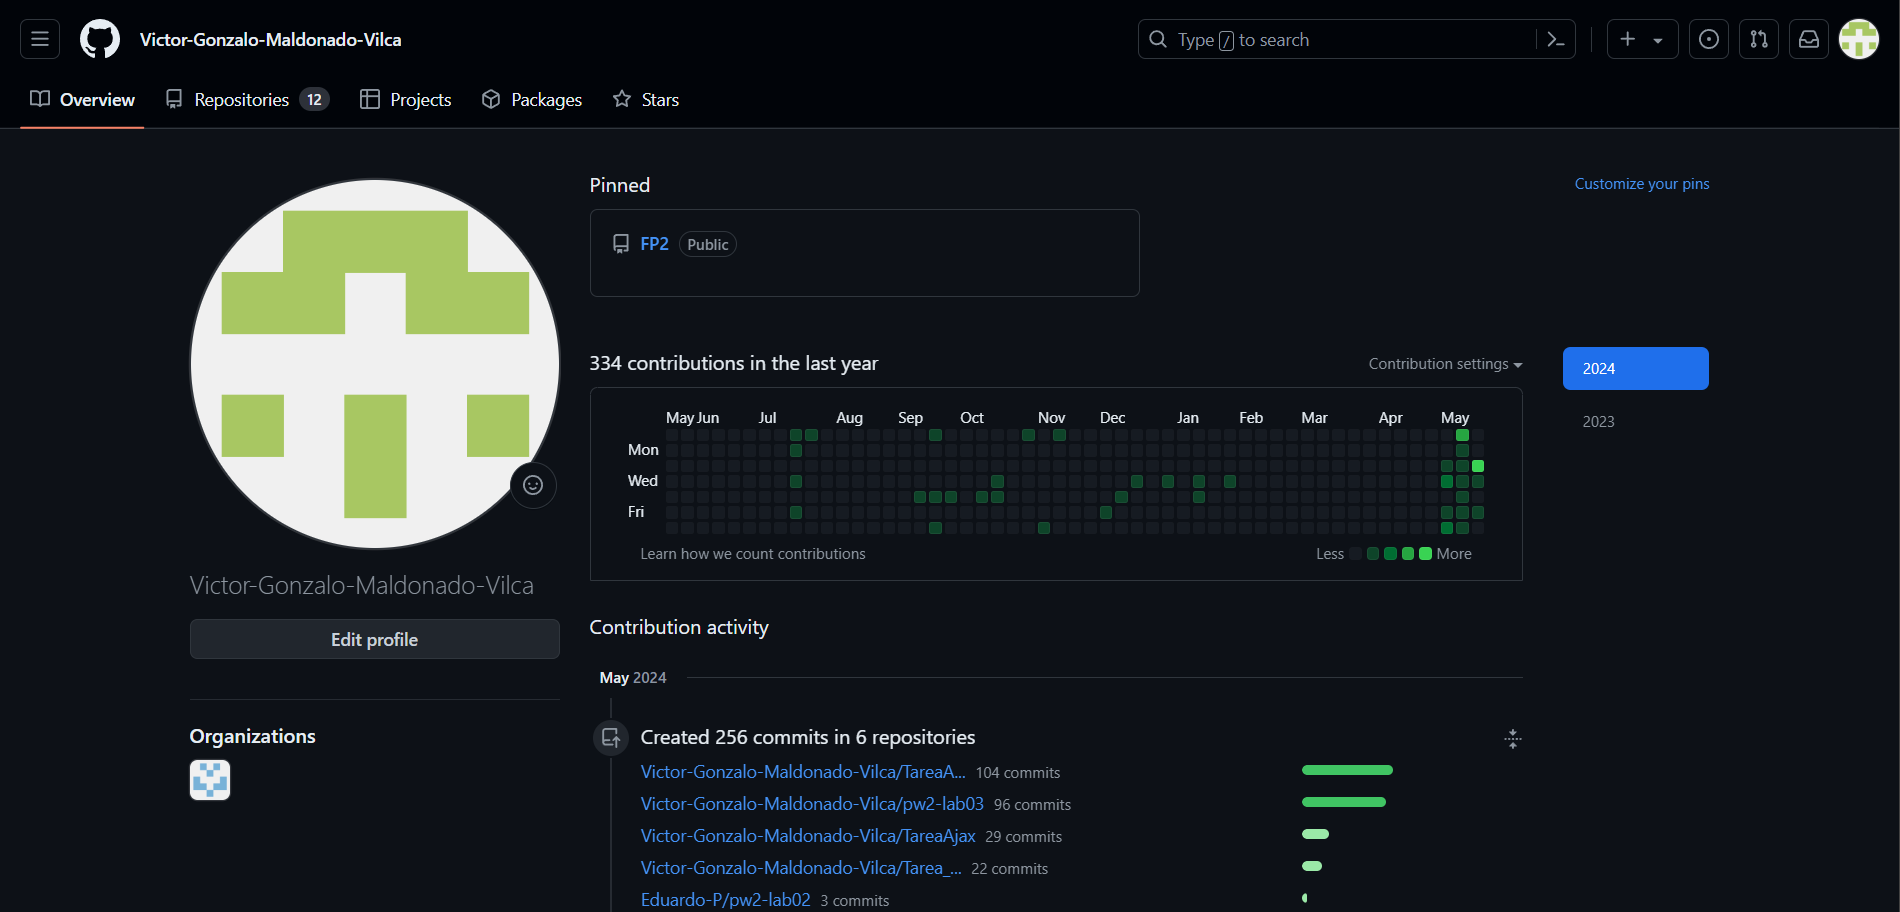
\includegraphics[width=1\textwidth, keepaspectratio]{img/usuario.png}
    \caption{Usuario}
  \end{figure}
  
%%%%%%%

  \subsubsection{Creación de un Nuevo Repositorio}
  \begin{figure}[H]
    \centering
    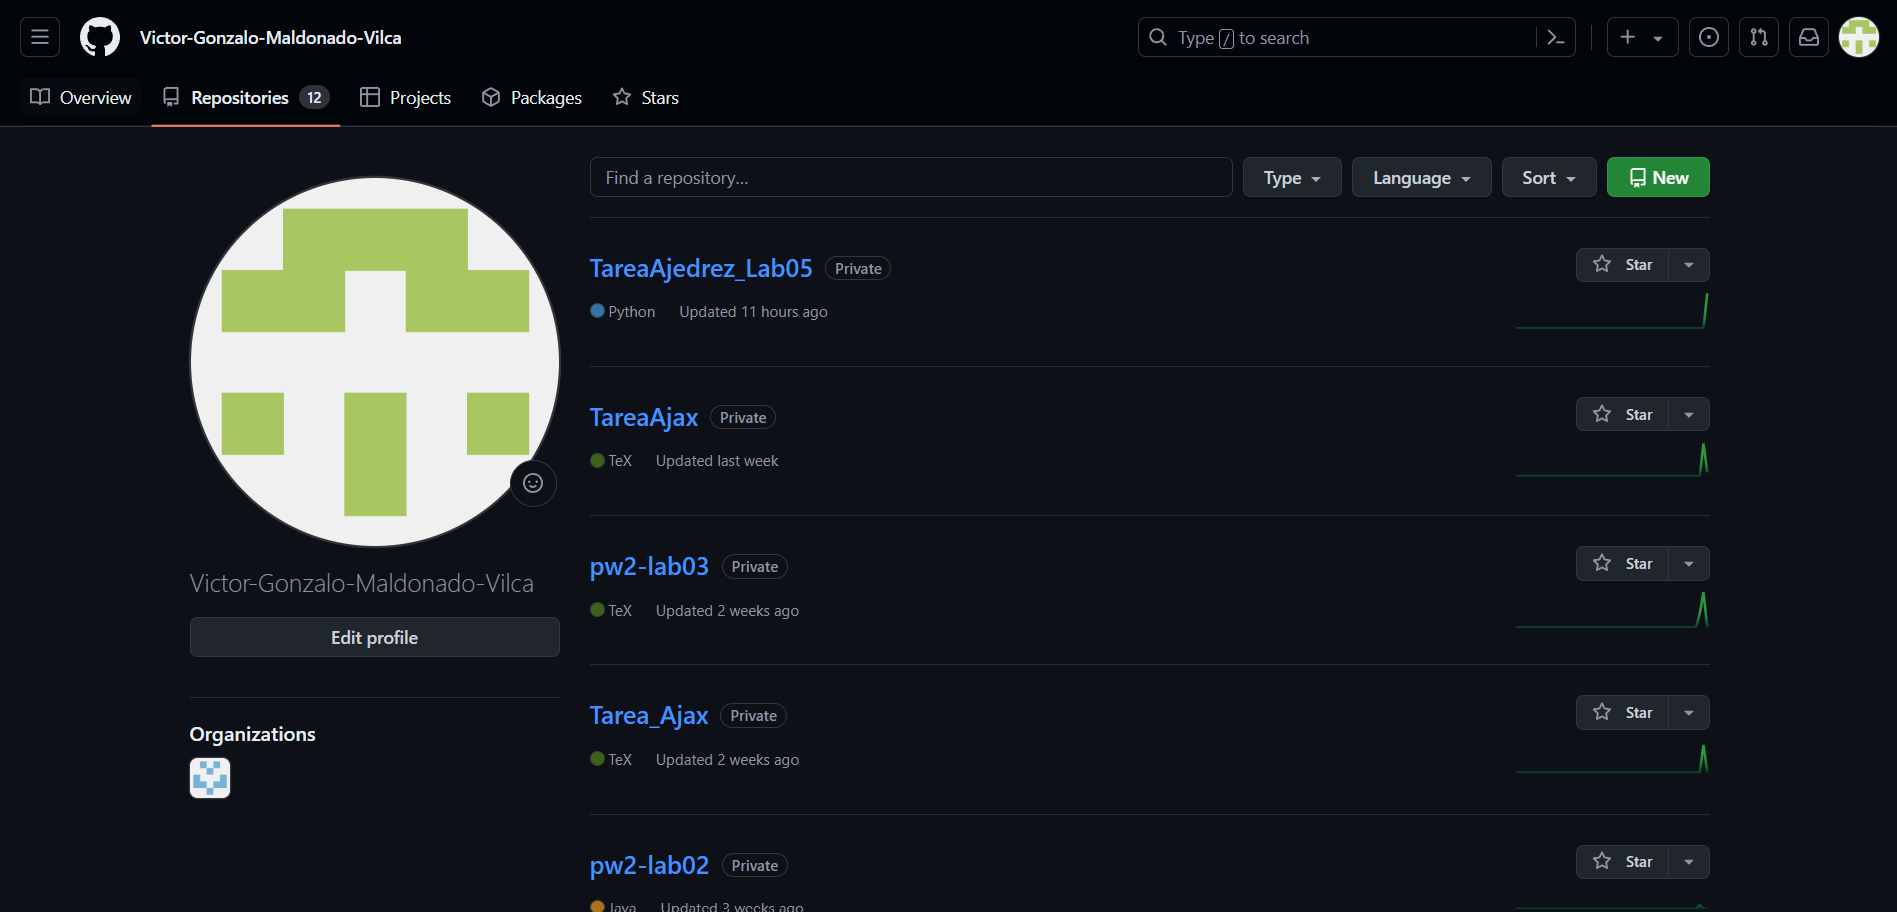
\includegraphics[width=1\textwidth, keepaspectratio]{img/creacion.png}
    \caption{Crear Repositorio \protect\texttt{TareaAjedrez\_lab05}}
  \end{figure}
  \newpage
  
%%%%%%%  
	
  \subsubsection{Comandos de Configuración}
  \begin{lstlisting}[language=, caption=Configuración Inicial]
    echo "# TareaAjedrez_lab05" >> README.md
    git init
    git add README.md
    git commit -m "first commit"
    git branch -M master
    git remote add origin https://github.com/Victor-Gonzalo-Maldonado-Vilca/TareaAjedrez_Lab05.git
    git push -u origin master
  \end{lstlisting}
  
%%%%%%%  
  
  \subsubsection{Implementación de Readme.md}
  \begin{figure}[H]
    \centering
    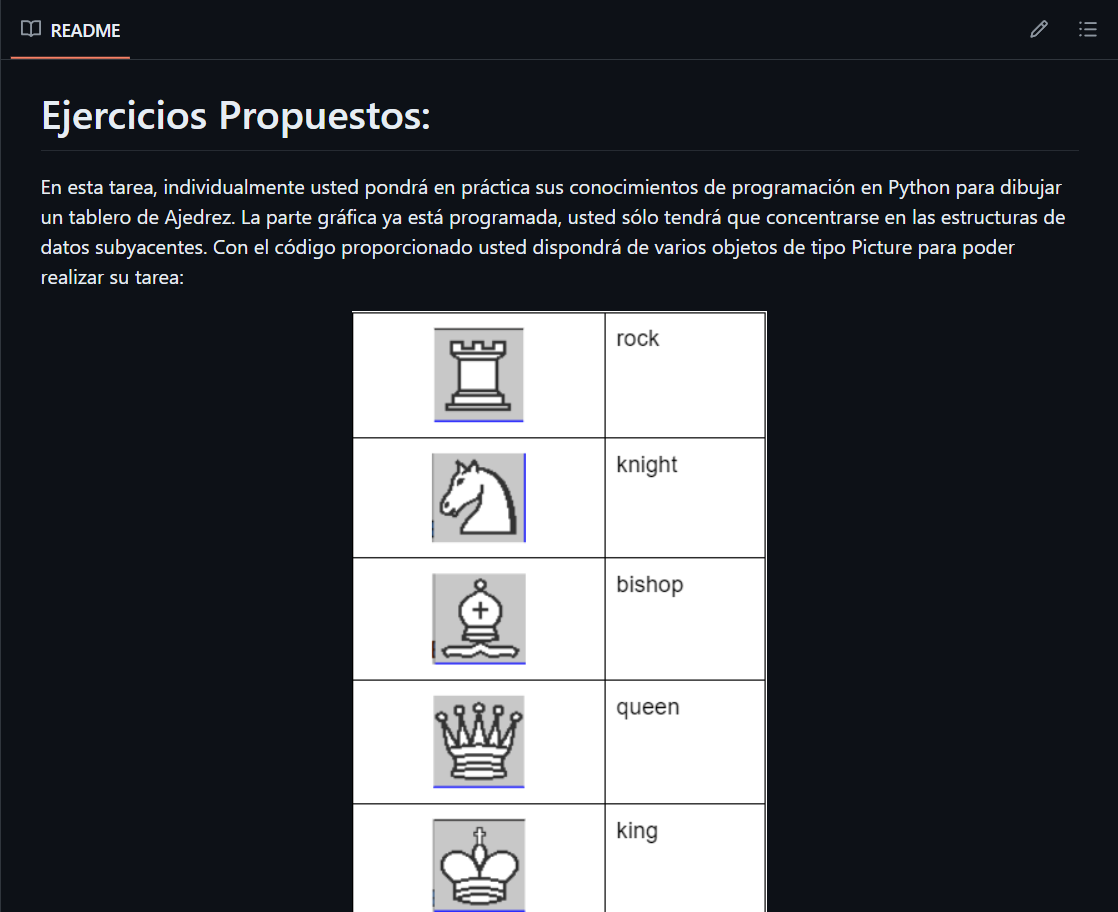
\includegraphics[width=1\textwidth, keepaspectratio]{img/readme.png}
    \caption{README.md}
  \end{figure}
  \newpage
  
%%%%%%%

	\subsubsection{Registro de cambios en mi código}
  \begin{figure}[H]
    \centering
    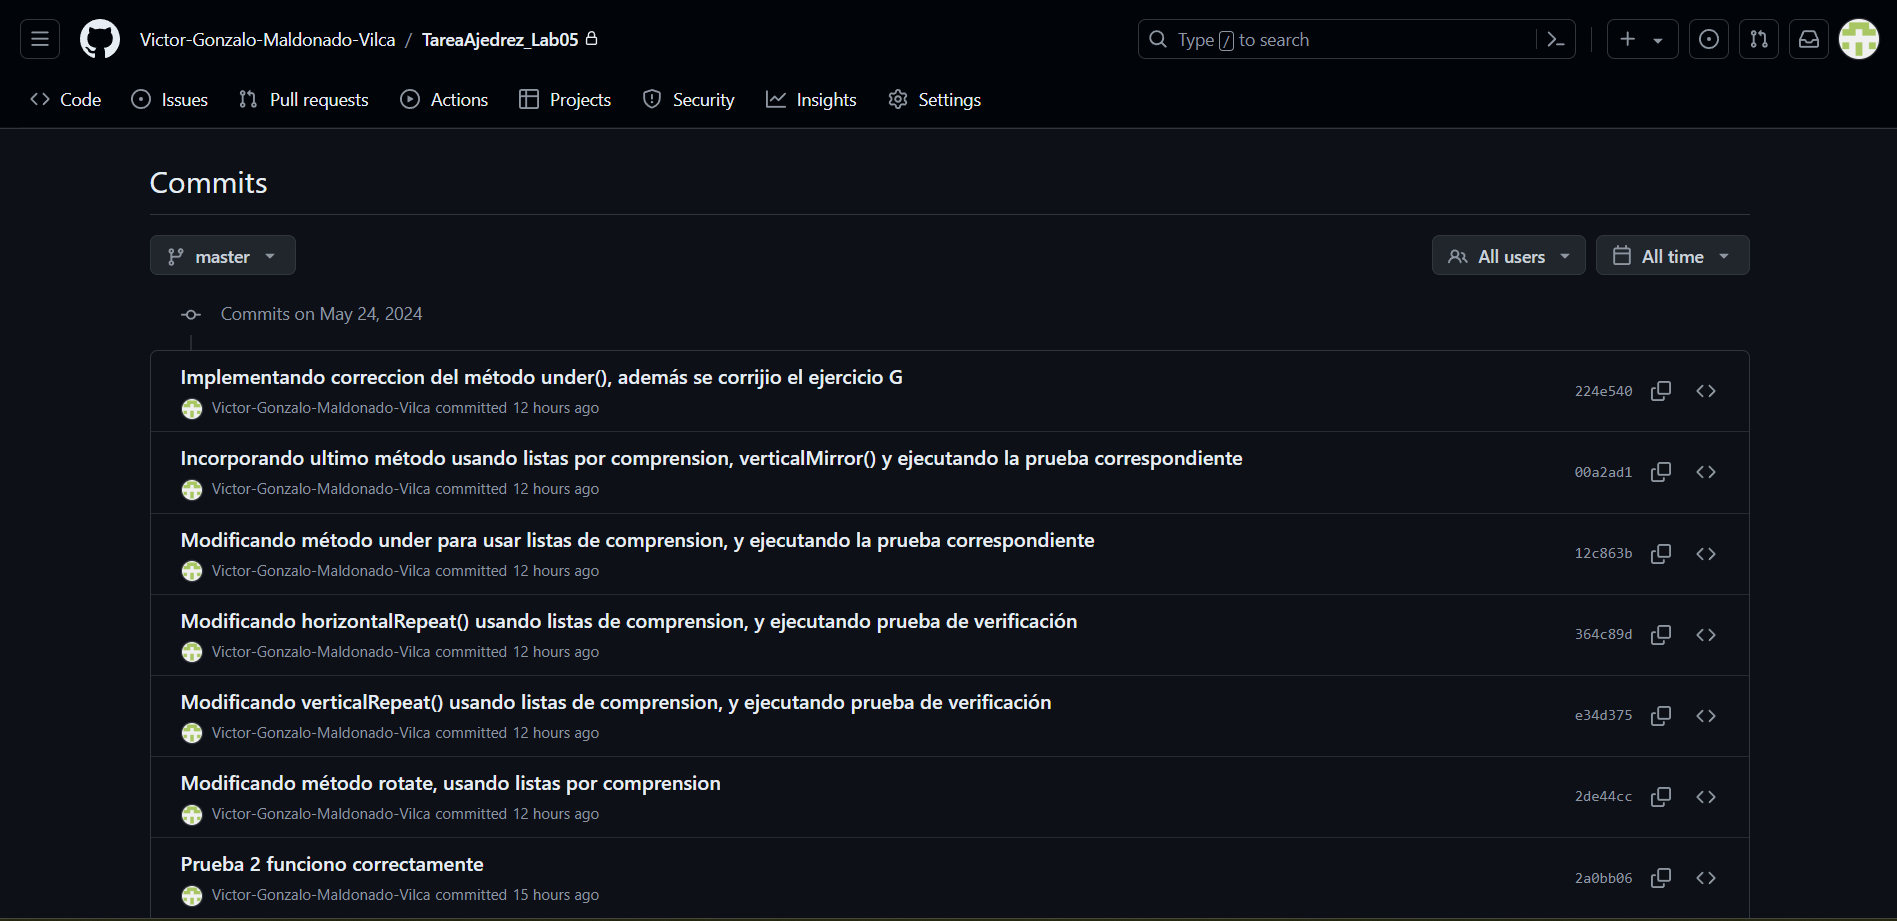
\includegraphics[width=1\textwidth, keepaspectratio]{img/commits.png}
    \caption{Commits}
  \end{figure}
	
%%%%%%%

	\subsubsection{Repositorio}
  \begin{figure}[H]
    \centering
    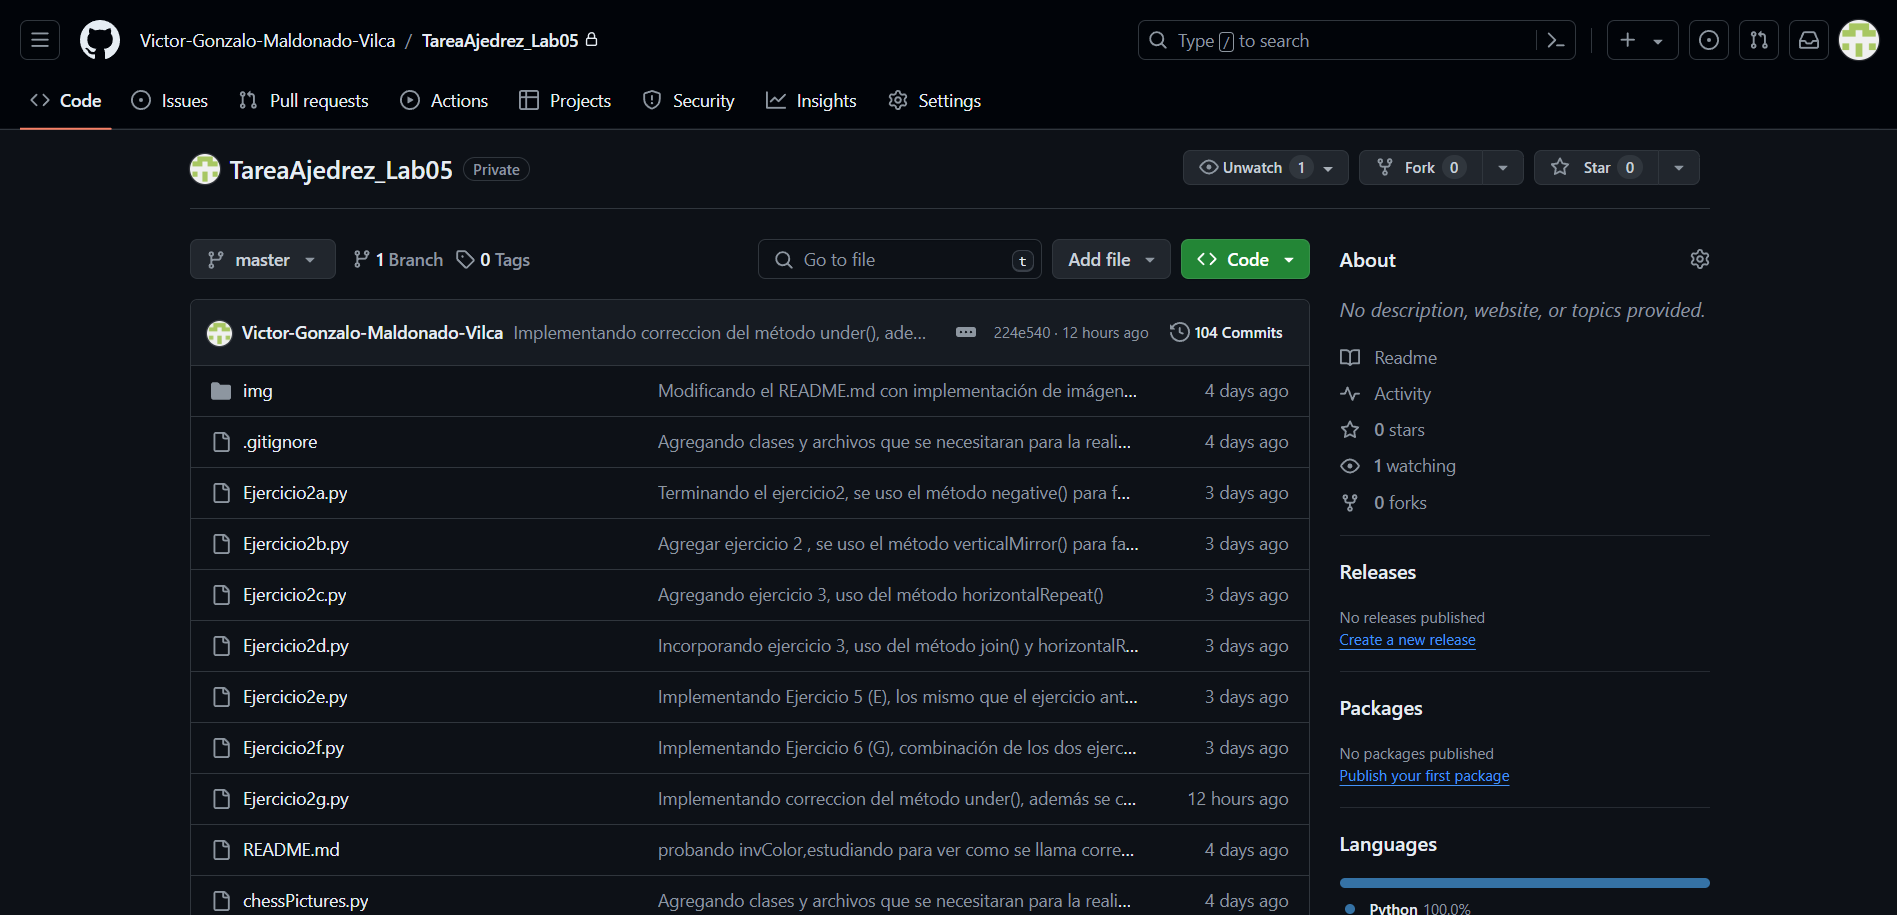
\includegraphics[width=1\textwidth, keepaspectratio]{img/Repositorio.png}
    \caption{Repositorio \protect\texttt{AjedrezTarea\_lab05}}
  \end{figure}
  \newpage
  
%%%%%%%

	\subsubsection{Proyecto compartido con el Docente de github}
  \begin{figure}[H]
    \centering
    \includegraphics[width=1\textwidth, keepaspectratio]{img/Compartir.png}
    \caption{Compartir con el Docente}
  \end{figure}
  
%%%%%%%%%%%%%%%%%%%%

  \section{Recomensaciones}
  \begin{itemize}
    \item Utilizar nombres de variables y funciones descriptivos para mejorar la legibilidad y comprensión del código.
    \item Aprovechar las características del lenguaje Python, como la comprensión de listas, generadores y decoradores, 
      para escribir código más eficiente y elegante.
    \item Utilizar entornos virtuales para aislar las dependencias de tus proyectos y evitar conflictos entre diferentes versiones de paquetes.
    \item Estudiar y experimentar para comprender mejor cómo trabajar con la clase Picture.
  \end{itemize}

%%%%%%%%%%%%%%%%%%%%

  \section{Conclusiones}
  \begin{itemize}
    \item La creación de entornos virtuales utilizando herramientas como virtualenv es fundamental para mantener un ambiente 
      de desarrollo limpio y aislado para cada proyecto.
    \item Pygame es una excelente opción para el desarrollo de juegos en Python, ofreciendo capacidades para crear interfaces 
      gráficas, manejar eventos de entrada y renderizar gráficos de manera eficiente.
    \item Picture es una biblioteca útil para la representación gráfica de figuras de ajedrez en Python, ofreciendo 
      funciones para cargar, procesar y renderizar estas figuras de manera eficiente.
  \end{itemize}

%%%%%%%%%%%%%%%%%%%%
	\newpage
	\subsection{\textcolor{red}{Rúbrica para el contenido del Informe y demostración}}
	\begin{itemize}			
		\item El alumno debe marcar o dejar en blanco en celdas de la columna \textbf{Checklist} si cumplio con el ítem correspondiente.
		\item Si un alumno supera la fecha de entrega,  su calificación será sobre la nota mínima aprobada, siempre y cuando cumpla con todos lo items.
		\item El alumno debe autocalificarse en la columna \textbf{Estudiante} de acuerdo a la siguiente tabla:
	
		\begin{table}[ht]
			\caption{Niveles de desempeño}
			\begin{center}
			\begin{tabular}{ccccc}
    			\hline
    			 & \multicolumn{4}{c}{Nivel}\\
    			\cline{1-5}
    			\textbf{Puntos} & Insatisfactorio 25\%& En Proceso 50\% & Satisfactorio 75\% & Sobresaliente 100\%\\
    			\textbf{2.0}&0.5&1.0&1.5&2.0\\
    			\textbf{4.0}&1.0&2.0&3.0&4.0\\
    		\hline
			\end{tabular}
		\end{center}
	\end{table}	
	

	\end{itemize}

 
	
	\begin{table}[H]
		\caption{Rúbrica para contenido del Informe y demostración}
		\setlength{\tabcolsep}{0.5em} % for the horizontal padding
		{\renewcommand{\arraystretch}{1.5}% for the vertical padding
		%\begin{center}
		\begin{tabular}{|p{2.7cm}|p{7cm}|x{1.3cm}|p{1.2cm}|p{1.5cm}|p{1.1cm}|}
			\hline
    		\multicolumn{2}{|c|}{Contenido y demostración} & Puntos & Checklist & Estudiante & Profesor\\
			\hline
			\textbf{1. GitHub} & Hay enlace URL activo del directorio para el  laboratorio hacia su repositorio GitHub con código fuente terminado y fácil de revisar. &2 &X &2 & \\ 
			\hline
			\textbf{2. Commits} &  Hay capturas de pantalla de los commits más importantes con sus explicaciones detalladas. (El profesor puede preguntar para refrendar calificación). &4 &X &4 & \\ 
			\hline 
			\textbf{3. Código fuente} &  Hay porciones de código fuente importantes con numeración y explicaciones detalladas de sus funciones. &2 &X &2 & \\ 
			\hline 
			\textbf{4. Ejecución} & Se incluyen ejecuciones/pruebas del código fuente  explicadas gradualmente. &2 &X &2 & \\ 
			\hline			
			\textbf{5. Pregunta} & Se responde con completitud a la pregunta formulada en la tarea.  (El profesor puede preguntar para refrendar calificación).  &2 &X &2 & \\ 
			\hline	
			\textbf{6. Fechas} & Las fechas de modificación del código fuente estan dentro de los plazos de fecha de entrega establecidos. &2 &X &2 & \\ 
			\hline 
			\textbf{7. Ortografía} & El documento no muestra errores ortográficos. &2 &X &2 & \\ 
			\hline 
			\textbf{8. Madurez} & El Informe muestra de manera general una evolución de la madurez del código fuente,  explicaciones puntuales pero precisas y un acabado impecable.   (El profesor puede preguntar para refrendar calificación).  &4 &X &4 & \\ 
			\hline
			\multicolumn{2}{|c|}{\textbf{Total}} &20 & &20 & \\ 
			\hline
		\end{tabular}
		%\end{center}
		%\label{tab:multicol}
		}
	\end{table}


%%%%%%%%%%%%%%%%%%%%%%%%%%%%%%%%%%%%%%%%%%%%%%%%%%%%%%%%%%%%%%%%%%%
	
  \newpage
  \section{Referencias}
  \begin{itemize}
    \item \url{https://www.python.org/}
    \item \url{https://www.pygame.org/news}
    \item \url{https://github.com/rescobedoq/pw2/tree/main/labs/lab04/Tarea-del-Ajedrez}
  \end{itemize}

%%%%%%%%%%%%%%%%%%%% 
%\clearpage
%\bibliographystyle{apalike}
%\bibliographystyle{IEEEtranN}
%\bibliography{bibliography}
			
\end{document}
